% This is samplepaper.tex, a sample chapter demonstrating the
% LLNCS macro package for Springer Computer Science proceedings;
% Version 2.20 of 2017/10/04
%
\documentclass[runningheads]{llncs}
%
\usepackage{graphicx}
\usepackage{amsmath}
%\usepackage{psfrag}
\usepackage{url}
\usepackage{rotating}
\usepackage{amsmath}
\usepackage{amsfonts}
\usepackage{amssymb}
\usepackage{subfigure}

\usepackage{xcolor}
\newcommand\anna[1]{\textcolor{red}{#1}}

% Used for displaying a sample figure. If possible, figure files should
% be included in EPS format.
%
% If you use the hyperref package, please uncomment the following line
% to display URLs in blue roman font according to Springer's eBook style:
% \renewcommand\UrlFont{\color{blue}\rmfamily}
\newcommand{\Bsep}{\: \mid \: }
\newcommand{\Rule}[2]{\displaystyle{\frac{#1}{#2}}}
\newcommand{\SF}[1]{\mathsf{#1}}
\newcommand{\Act}{\mathsf{Act}}
\newcommand{\Vis}{\mathsf{Vis}}
\newcommand{\ActK}{\mathsf{ActK}}
\newcommand{\Proc}{\mathsf{Proc}}
\newcommand{\Var}{\mathsf{Var}}
\newcommand{\Procc}{\mathsf{ProcC}}
\newcommand{\Pred}{\mathsf{Pred}}
\newcommand{\Std}{\mathsf{Std}}
\newcommand{\rms}{\mathrm{S}}
\newcommand{\rmrec}{\mathrm{rec}}
\newcommand{\rmreck}{\mathrm{reck}}
\newcommand{\rmreckR}{\mathrm{reckR}}
\newcommand{\rma}{\mathrm{A}}
\newcommand{\rmp}{\mathrm{P}}
\newcommand{\rmf}{\mathrm{F}}
\newcommand{\rmr}{\mathrm{R}}
\newcommand{\rmfr}{\mathrm{FR}}
\newcommand{\equivS}{\equiv_{\mathrm{S}}}
\newcommand{\SigSA}{\Sigma_{\mathrm{SA}}}
\newcommand{\ltran}[1]{\stackrel{#1}{\longrightarrow}}
\newcommand{\tran}[1]{\stackrel{#1}{\rightarrow}}
\newcommand{\Tran}[1]{\stackrel{#1}{\Rightarrow}}
\newcommand{\nottran}[1]{\stackrel{#1}{\not\rightarrow}}
\newcommand{\Rtran}[1]{\stackrel{#1}{\rightsquigarrow}}
\newcommand{\notRtran}[1]{\stackrel{#1}{\not\rightsquigarrow}}
\newcommand{\trans}[1]{\stackrel{#1}{\rightarrow}_{\mathrm{S}}}
\newcommand{\Par}{\mid}
\newcommand{\restrict}[1]{\!\setminus\!#1}
\newcommand{\paral}{\; \vert \;}

\newcommand{\mA}{\mathcal{A}}
\newcommand{\mSA}{\mathcal{SA}}
\newcommand{\mWA}{\mathcal{WA}}
\newcommand{\mAK}{\mathcal{AK}}
\newcommand{\aAK}{\mathcal{(A)K}}
\newcommand{\umAK}{\underline{\mathcal{A}}\mathcal{K}}
\newcommand{\un}[1]{\underline {#1}}
\newcommand{\PI}{\mathcal{PI}}
\newcommand{\rom}[1]{\mbox{\rm{#1}}}

\newcommand{\Nil}{\mathbf{0}}
\newcommand{\New}[1]{\nu#1\: }
\newcommand{\Str}{\equiv}
\newcommand{\stdpred}{\mathsf{std}}
\newcommand{\std}[1]{\mathsf{std}(#1)}
%
\newcommand{\Bch}[2]{\mathsf{before}_{#1}(#2)}

\newcommand{\keys}[1]{\mathsf{keys}(#1)}
\newcommand{\kkey}[1]{\mathsf{k}(#1)}
\newcommand{\key}[1]{[#1]}
\newcommand{\Keys}{\mathcal{K}}
\newcommand{\Subscripts}{\mathcal{S}}
\newcommand{\freshpred}[1]{\mathsf{fsh}[#1]}
\newcommand{\fresh}[2]{\mathsf{fsh}[#1](#2)}
\newcommand{\freshsubscript}[2]{\mathsf{fshsubscript}[#1](#2)}
\newcommand{\subscript}[1]{\mathsf{s}(#1)}

\newcommand{\alphaconversionkey}[3]{\mathsf{\alpha keys}(#1,#2,#3)}
\newcommand{\alphaconversionkeyk}[3]{\mathsf{\alpha k}(#1,#2,#3)}
\newcommand{\alphaconversionsub}[3]{\mathsf{\alpha subscripts}(#1,#2,#3)}
\newcommand{\alphaconversionsubs}[3]{\mathsf{\alpha s}(#1,#2,#3)}
\newcommand{\alphaconversionsubsr}[3]{\mathsf{\alpha sr}(#1,#2,#3)}
\newcommand{\alphaconversionsubsc}[3]{\mathsf{\alpha sc}(#1,#2,#3)}

\newcommand{\ta}[1]{\mathsf{ta}(#1)}
\newcommand{\action}[1]{\mathsf{act}(#1)}

\newcommand{\intr}{\mbox{\ $\hat{}$\ }}
%\newcommand{\intr}{\mbox{\; $\widehat{}$\;}}
\newcommand{\sterm}{\mathsf{trm}}
\newcommand{\Sterm}[1]{\sterm(#1)}
\newcommand{\und}[1]{\underline{#1}}
\newcommand{\sqc}{\mathop{\cdot}}
\newcommand{\card}[1]{|#1|}
\newcommand{\bydef}{\stackrel{\emph{def}}{=}}
%
\newcommand{\Angle}[1]{\langle #1 \rangle}
\newcommand{\Tri}{\triangleright}
\newcommand{\Hole}{\bullet}
\newcommand{\rec}[1]{\mathrm{rec}\, #1}
\newcommand{\Rec}[1]{\rec #1 .}
\newcommand{\Rch}{\mathsf{Rch}}
\newcommand{\prune}{\pi}
\newcommand{\Prune}[1]{\prune(#1)}
\newcommand{\Root}[1]{\mathsf{rt}(#1)}
\newcommand{\hole}{\mbox{$[\ ]$}}

\newcommand{\Bis}{\sim}
\newcommand{\Biss}{\Bis_{\mathsf{S}}}
\newcommand{\Bisf}{\Bis_{\mathsf{F}}}
\newcommand{\Bisfr}{\Bis_{\mathsf{FR}}}
%\newcommand{\Bisu}{\Bis_{\Un}}
\newcommand{\Sim}{\mathcal{S}}
\newcommand{\Rem}{\backslash}
\newcommand{\sqeqt}{\sim}
% rules:
% static rule
\newcommand{\one}{\mbox{(I)}}
\newcommand{\onef}{\mbox{(1)}}
\newcommand{\oner}{\mbox{(1R)}}
% choice rule
\newcommand{\two}{\mbox{(II)}}
\newcommand{\twof}{\mbox{(2)}}
\newcommand{\twor}{\mbox{(2R)}}
% choice axiom
\newcommand{\thr}{\mbox{(III)}}
\newcommand{\thrf}{\mbox{(3)}}
\newcommand{\thrr}{\mbox{(3R)}}
\newcommand{\thrpf}{\mbox{(3\,$'$\!)}}
\newcommand{\thrpr}{\mbox{(3\,$'$\!R)}}
%
%
\newcommand{\Draft}[1]{}
\newcommand{\Comment}[1]{}
\newcommand{\Rev}[1]{{#1}^{-1}}
\newcommand{\Stefan}[1]{{\bf S(} #1 {\bf )S}}
\newcommand{\rulename}[1]{\textsf{#1}}

\newcommand{\A}{\mathcal{A}}
\newcommand{\B}{\mathcal{B}}
\newcommand{\N}{\mathbb{N}}
\newcommand{\mN}{\mathcal{N}}
\newcommand{\mM}{\mathcal{M}}
\newcommand{\mP}{\mathcal{P}}
\newcommand{\I}{\mathcal{I}}
\newcommand{\Q}{\mathbb{Q}^+}
\newcommand{\C}{\mathcal{C}}
\newcommand{\R}{\mathbb{R}}
\newcommand{\MolOxy}{\mathit{MolOxy}}
\newcommand{\MolHy}{\mathit{MolHy}}
\newcommand{\Uppaal}{{\scshape Uppaal}\,}

\newcommand{\PN}{reversing Petri net } 
\newcommand{\guard}[1]{\mathsf{pre}(#1)}
\newcommand{\effects}[1]{\mathsf{post}(#1)}
\newcommand{\bond}{\!-\!}
\newcommand{\connected}{\mathsf{con}}
\newcommand{\state}[2]{\langle {#1}, {#2}\rangle}
\newcommand{\rtrans}[1]{\ensuremath{\stackrel{#1}{\rightsquigarrow}}}
\newcommand{\RPN}{\textsc{RPN\ }} 
\newcommand{\type}{\mathit{type}}
\begin{document}
%
\title{Reversibility in chemical reactions\thanks{The authors acknowledge partial support of COST Action IC1405 on Reversible Computation - extending horizons of computing.}}
%
%\titlerunning{Abbreviated paper title}
% If the paper title is too long for the running head, you can set
% an abbreviated paper title here
%
\author{Stefan Kuhn\orcidID{0000-0002-5990-4157}\inst{1}, Bogdan Aman\orcidID{0000-0001-7649-8181}\inst{2,3}, Gabriel Ciobanu\orcidID{0000-0002-8166-9456}\inst{2,3},  Anna Philippou\inst{4}, Kyriaki Psara\inst{4}, and  Irek Ulidowski\inst{5}}
%
\authorrunning{S. Kuhn et al.}
% First names are abbreviated in the running head.
% If there are more than two authors, 'et al.' is used.
%
\institute{School of Computer Science and Informatics, De Montfort University, Leicester, UK\\ \email{\scriptsize stefan.kuhn@dmu.ac.uk} \and
Romanian Academy, Institute of Computer Science, Ia\c si\\
 \email{\scriptsize bogdan.aman@iit.academiaromana-is.ro, gabriel@info.uaic.ro } \and
A.I.Cuza University, Faculty of Computer Science, Ia\c si, Romania\\ 
\and
Department of Computer Science, University of Cyprus \\ \email{\scriptsize \{annap,kpsara01\}@cs.ucy.ac.cy}  \and 
Department of Informatics, University of Leicester\\ 
\email{\scriptsize iu3@leicester.ac.uk} 
}
%
\maketitle              % typeset the header of the contribution
%
\begin{abstract}
In this chapter we give an overview of some techniques developed for modelling and reasoning about reversibility of systems, including out-of-causal-order reversibility, as this appear for example in chemical reactions. We use the autoprotolysis of water as an example. We model this using the Calculus of Covalent Bonding (CCB), the Bonding Calculus, and Reversing Petri Nets (RPNs), thus demonstrating the use of the three formalisms while contrasting them to CCS with keys (CCSK), a conventional reversible process calculus. This exercise demonstrates that these formalisms, developed  especially for the purpose of expressing advanced forms of reversibility, are able to model the reaction more accurately. At the same time, each formalism has its own characteristics and expressiveness potential, which are brought out in our discussion.

\keywords{ Reversibility \and Reaction Modelling \and Process calculi \and Bonding Calculus \and Calculus of Covalent Bonding \and Reversing Petri Nets }
\end{abstract}
%
%
%
\section{Introduction}

Biological reactions, pathways and reaction networks have been extensively studied in the literature using
various  techniques,  including  process  calculi and Petri nets.  Initial research was mainly focused  on
reaction rates by modelling and simulating networks of reactions, in order to
analyse or even predict the common paths through the network.  Reversibility
was not considered explicitly.  Later on
reversibility  started  to  be  taken  into  account,  since  it  plays  a  crucial  role  in
many processes, typically by going back to a previous state in the system.  For
example,  reversibility is needed to model directly when a gene is regulated by a protein binding to it and unbinding from it.  Such examples can
be modelled by backtracking the computation along the executed path of action that led to the current state.  Beyond
backtracking and causal reversibility, there is a more general form of reversibility, known as out-of-causal-order reversibility, which makes it possible to get
to states which cannot be reached by forward reactions alone.  Such sequences
of forward and reversible reactions are important as they lead to new chemical
structures and new reactions, which would not be possible without out-of-causal-order
reversibility.

Looking at proteins and other macromolecules means working at relatively
high  levels  of  abstraction.   It  also  means  that  such  biological  entities  are  often  difficult  to  represent  as  there  is  still  no  complete  understanding  of  their
behaviour.  Also their interactions with other similar molecules are hard to enumerate as they are sometimes not fully understood. This could also mean that some aspects of reversibility are not clearly modelled since  too  much
detail is abstracted away. Therefore,  new modelling techniques are needed in order to capture reversible behavior when studying biological systems. In this chapter, we present techniques to this effect and concentrate on chemical reactions, a domain that offers
interesting examples of out-of-causal-order reversibility. %we  have studied chemical  reactions  when studying reversibility in the context of living systems. We have done this using techniques which have mostly been applied to higher-level biological systems. This is justified since chemical reactions involve various forms of reversibility and offer good case
%studies  for  the  modelling  of  reversibility. Specifically,  we  can  find  interesting
%examples  of  the  out-of-causal  order  reversibility  in  many  chemical  reactions,
%and can 
The presented techniques enable one to model the intermediate steps of such reactions where some bonds are
only ``helping'' to achieve the overall aim of the reaction:  specifically, they are only formed to be
broken before the end of the reactions.  Thus, the allowed level of detail 
%we have on
%chemical  reactions  makes more obvious the use of  reversibility compared to higher level models.  In many cases we have the additional benefit of good
makes a more accurate depiction of the reversibility in place, and allows a more thorough understanding of the underlying reaction mechanisms 
compared to higher-leverl models.


Process calculi, originally designed for modelling concurrent computations, have been applied to model biochemical and biological systems. We can mention the $\pi$-calculus \cite{MilnerPi,Regev2004}, BioAmbients \cite{RegevBioambients}, the stochastic $\pi$-calculus \cite{PriamiStochasticPi}, beta binders~\cite{betabinders} and bioPEPA \cite{CiocchettaBiopepa}. These approaches allow to model various biological entities (e.g., molecules, proteins) as interacting processes when describing a complex system. The process calculi are compositional, and so they allow to explicitly model the activity of the whole complex system by composing the activities of some smaller entities. Each term in the description of such a system has a counterpart in the biophysical system, and the behaviour of the whole system is obtained by following the operational semantics of the process calculi. On the other hand, the bonding calculus \cite{NaCo18} is different from these approaches mentioned above.  \anna{In this last sentence and the following paragraphs there is specific mention on the bonding calculus or CCB (I will highlight some such points). A simultaneous reference to CCB/bonding calculus would be useful. At some point, possibly the conclusions, it might be good to make a more careful comparison between the two, both being process calculi.} In BioPEPA the abstraction ``processes as species'' is used by considering the concentrations of the involved processes. In the other calculi,  the abstraction ``processes as interactions'' is used similar as in bonding calculus, but processes are able to communicate values in order to interact (this is not the case in the bonding calculus). 


Another approach to model biological interactions is by using rule-based formalisms such as BIOCHAM \cite{biocham}, the $\kappa$-calculus  \cite{danoscausality} and the BioNetGen Language (BNGL) \cite{pmid19399430}. Just like in bonding calculus, $\kappa$ and BNGL formalisms can be used to model interactions between proteins, while this is not true in BIOCHAM. Just like in BNGL, bonding calculus allows the use of molecule sites having the same name, while this is not possible in the $\kappa$-calculus. While the $\kappa$-calculus describes molecules as a set of sites and uses rules to manipulate these sites between two or more molecules, in the  bonding calculus \cite{NaCo18} a molecule is described by the sequence of operations it can perform on its sites (including also non-deterministic choices), regardless of the form of the other molecules. This allows to use the compositionality of the process calculus. Moreover, the number of rules is smaller in bonding calculus due to the use of generic rules.

Most of the formalisms mentioned do not explicitly deal with reversibility. If an action is the reverse of something done before, there is no explicit knowledge of that in the model. Attempts at modelling reversibility in process calculi are CCSK \cite{Irek2007} and RCCS \cite{danos2004ccsr}. Both are based on the Calculus of Communicating Systems (CCS) \cite{MilnerBook}. They extend CCS by keeping track of past actions and enabling an undo of those. So a reverse action is the reverse execution of the forward action, which is not the case in other calculi. Actions can be undone in exactly the reverse order as they were executed forward (backtracking) or in a causally-consistent order, which can be different from the forward execution, as long as effects are undone before their causes. The \anna{Calculus of Covalent Bonding} (CCB) \cite{KUHN201818} enables the modelling of out-of-causal-order reversibility. In biological and chemical systems such seemingly out-of-causal-order executions are commonly observed. Since \anna{CCB} models chemical reactions closely, it can generate such behaviour. It should be emphasized that this is visible at a certain level of detail, whilst there is no causality in a more detailed view. This suggests that this is a case of emergent behaviour.

Petri nets (PNs)~\cite{PNs} are another formalism that has been widely used to model and reason
about a wide range of applications featuring concurrency and distribution. They are a graphical 
language  associated with 
a rich mathematical theory and supported by a variety of tools. Their employment in systems 
biology was initiated in~\cite{DBLP:conf/ismb/ReddyML93,DBLP:journals/jsamas/HofestadtH94}
and since then they have been widely employed for
the modelling, analysis, and simulation of a diversity of biological systems including 
biochemical reactions in metabolic pathways, gene expression, signal transduction, and neuronal processes~\cite{PNbiology,DBLP:journals/bib/Chaouiya07,DBLP:journals/nc/BaldanCMS10}. Indeed, PNs seem to be a natural framework for representing biochemical systems as themselves constitute a set of interdependent
transitions/reactions which consume 
and produce resources, and are represented graphically in a similar fashion to the systems
in question. Furthermore, a PN model
can be decomposed in order to handle the overall complexity, and the abstraction level of a model
can vary from single molecules, to cells, to multicellular aggregations.
Several specialized Petri net classes like qualitative, stochastic, continuous, or
hybrid Petri nets and their coloured counterparts have been used to describe different
systems~\cite{DBLP:journals/jamia/PelegRA05,DBLP:journals/isb/HofestadtT98,DBLP:journals/fuin/Popova-ZeugmannHK05,DBLP:journals/nc/MatsunoNM11,DBLP:journals/isb/VossHK03}.
At the same time, PNs enable a wide range of analysis techniques, 
such as determining states of equilibrium, conflicting evolutions, 
and reachable states. 

As far as reversibility is concerned, classical PNs and their extensions do not
directly handle reversibility. Modelling reversible reactions in these formalisms requires the employment
of mechanisms involving two distinct transitions,
one for the forward and one for the reverse version of a reaction. This
may result in expanded models and state spaces and less natural and/or less accurate
models of  reversible behavior. In this study we consider
a recently-introduced extension of Petri nets called reversing Petri nets (RPNs)~\cite{RPNs}.
%A large amount of work has focused on providing a formal understanding of reversibility within process calculi and it has recently been extended to the formalism of Petri nets.  
%Petri nets (PNs)~\cite{PNs} are a graphical mathematical language that can be used for the specification and
%analysis of discrete event systems. 
%The first study of reversible computation within PNs was proposed in~\cite{PetriNets,BoundedPNs}. In these works, the
%authors investigate the effects of adding \emph{reversed} versions of selected transitions in a PN
%by reversing the directions of a transition's arcs. They then explore decidability problems regarding reachability and coverability in the resulting PNs. In
%was proposed, called reversing Petri nets (RPNs).  In this work, RPNs are acyclic Petri net structures that  assume 
RPNs are the first proposal for capturing reversible behavior directly in the Petri net model
and they support reversible computation in all its forms
(backtracking, causal-order reversibility and out-of-causal-order reversibility).
RPNs  enable the reversal of each executed transition and assume tokens to be distinguished from each 
other by an identity/type and to be persistent. Furthermore,
during transitions tokens can be bonded together, with  the creation of bonds
 considered to be the effect of a transition, whereas their destruction is the effect of
the transition's reversal. The notion of bonds is especially useful for reasoning about biochemical
systems as illustrated in the current paper. % through the case study of the autoprotolysis of water.
RPNs have been shown to be closely related to Coloured Petri Nets, as a subset of the former model
has been encoded into the latter~\cite{RPNtoCPN}.
%RPNs
%have been extended with cycles~\cite{RPNJournal} and with a mechanism for controlling transition
%reversal by associating transitions with conditions~\cite{RC19}. 

\section{The autoprotolysis of water}

We consider a reaction that transfers a hydrogen atom between two water molecules. Since the
reaction takes place in water it is also known as \emph{autoprotolysis of water}. The reaction is shown 
in Figure~\ref{fig:autoprotolysis}. Here, $O$ indicates an oxygen atom and $H$ a hydrogen atom. The lines indicate bonds. Charges on atoms are shown by $\oplus$ and $\ominus$. The meaning of the curved arrows and the dots will be explained in the next paragraph. The reaction is reversible and it takes place at a relatively 
low rate, making pure water slightly conductive.

\begin{figure}
\centering
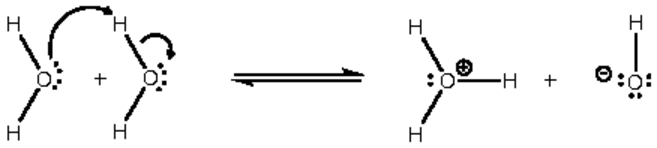
\includegraphics[height=1.5cm]{autoprotolysis_corr3}
\caption{Autoprotolysis of water.}
\label{fig:autoprotolysis}
\end{figure}

In order to model this reaction we need to understand its causes. % what it is that makes it happen.
The main factor is that the oxygen in the water molecule is \emph{nucleophilic}, meaning it has the tendency to bond to another atomic nucleus, which would serve as an \emph{electrophile}. This is because oxygen has a high 
electro-negativity, therefore it attracts electrons and has an abundance of electrons around it. The electrons around the atomic nucleus are arranged on electron shells, where only those in the outer shell participate in bonding. Oxygen has four electrons in its outer shell, which are not involved in the initial bonding with hydrogen atoms. These electrons form two \emph{lone pairs} of two electrons each, which can form new bonds (lone pairs are shown in Figure~\ref{fig:autoprotolysis} by pairs of dots). All this makes oxygen nucleophilic: it tends to connect 
to other atomic nuclei by forming bonds from its lone pairs. Since oxygen attracts electrons, the hydrogen atoms in water
have a positive partial charge and oxygen has a negative partial charge. 

The reaction
starts with an oxygen (in one water molecule) being attracted by a hydrogen in another 
water molecule due to their opposite
charges (this attraction is called a \emph{hydrogen bond}). Due to the nucleophilicity of 
the oxygen, a bond can form to the hydrogen. This bond is formed out of 
the electrons of one of the lone pairs of the oxygen. The curved arrows in Figure~\ref{fig:autoprotolysis} indicate the movements of the electrons. Since a hydrogen atom cannot have more 
than one bonds, 
the creation of a new bond is compensated by breaking the existing hydrogen-oxygen bond (again indicated by a curved arrow
\anna{perhaps use another color for this arrow to distinguish? stefan I don't think we can use color}anna: Perhaps then a different type of arrow?). When this happens, the two electrons, which formed the original hydrogen-oxygen bond, remain with the oxygen. Since a hydrogen contains %consists of 
one electron and one proton, it is only the proton that is transferred, so the process can be called a proton transfer as well as a hydrogen transfer. The forming of the new bond and the breaking of the old bond are concerted, meaning that %namely
they happen together without a stable 
intermediate configuration. As a result we have reached the state where one oxygen atom
has three bonds to hydrogen atoms and is positively charged, represented on the right side of the reaction in %of
 Figure~\ref{fig:autoprotolysis}. This molecule is called hydronium and is written as $\mathrm{H_3O^+}$. The other oxygen atom bonds to only one hydrogen and is negatively charged, having an 
electron in surplus. This molecule is called a hydroxide and is written as $\mathrm{OH^-}$. 

We notice the reaction is reversible: the oxygen, which has lost a hydrogen, can 
pull back one of the hydrogens from the other molecule, the  $\mathrm{H_3O^+}$ molecule. This is the case since the negatively 
charged oxygen is a strong nucleophile and the hydrogens in the $\mathrm{H_3O^+}$ molecule are 
all positively charged. Therefore, any of the hydrogens 
%(not just the one which moved in the first instance) 
can be removed, making both oxygens formally uncharged, and restoring the two water 
molecules. In Figure~\ref{fig:autoprotolysis} the curved arrows are given for the reaction going from left to right. Since the reaction is reversible (indicated by the double arrow) there are correspondent electron movements when going from right to left. These are not given in line with usual conventions, but can be inferred.

In this simple reaction, the forward and the reverse step consist of two steps each. The breaking of the old and the forming of the new bond occur simultaneously. This means that there is no strict causality of actions, since none of them can be called the cause of the overall reaction. Furthermore, the reverse step can be done with a different atom to the one used during the forward step because each of the molecules are in a sense identical and in practice there does not exist a single ``reverse'' path corresponding to a forward one.%it is difficult to identify a  clear forward and reverse path. 

It should be noted that there are two types of bonding modelled here. Firstly, we have the initial bonds where two atoms contribute an electron each. Secondly, the \emph{dative or coordinate bonds} are formed where both electrons come from one atom (an oxygen in this case). Both are \emph{covalent bonds}, and once formed they cannot be distinguished. Specifically, in the oxygen with three bonds all bonds are the same and no distinction can be made. If one of the bonds is broken by a deprotonation (as in the autoprotolysis of water) the two electrons are left behind and they form a lone pair. If the broken bond was not previously formed as a dative bond, the electrons changed their ``role''. This explains why any proton can be transferred in the reverse reaction and not just the one involved in the forward path.

\section{Existing reversible formalisms}
In order to see how accurately existing formalisms can capture the autoprotolysis of water, we model it in CCS with keys (CCSK) \cite{Irek2007}. CCSK is a variation of the Calculus of Communicating Systems which includes reversibility. 

\subsection{Syntax of CCSK}

The key idea of CCSK is to extend CCS to mark past actions with a key instead of discarding them. These keys can then be used to undo actions. The syntax is an extension of CCS, so every CCS process is a valid CCSK process as well. We illustrate the working of CCSK with an example. The process
%
$$a.\Nil \paral b.\Nil$$
%
is ready to perform $a$ or $b$, just like a CCS process. If we execute $a$, we get
%
$$a[1].\Nil \paral b.\Nil$$
%
where $1$ is a key. $a$ is now a past action. The process could next do $b$ and we get
%
$$a[1].\Nil \paral b[2].\Nil$$
%
At this point, we now have the choice of undoing either $a$ or $b$. If we undo $b$, we get
%
$$a[1].\Nil \paral b.\Nil$$
%
which is the same as the process after performing $a$, so we reversed back to this state. We could also have undone $b$ instead, which would have been a causally-consistent path, but not backtracking. The semantics of CCSK are specified by SOS rules (see \cite{Irek2007}), which are the reverse of the forward CCS rules.

\subsection{The autoprotolysis of water in CSSK}

To model the system of two water molecules in CCSK, we would model oxygen and hydrogen atoms with appropriate actions. The modelling most faithful to the real situation is this:

%
$$\begin{array}{lll}
H & \bydef & \overline{a}.H'\\
O & \bydef & a.a.a.O'
\end{array}$$
%
where $H'$ and $O'$ are synonyms of $\Nil$ and help to identify processes. Here, an oxygen atom is modelled with three prefixes and a hydrogen atom with the corresponding co-name. As in CCS, these can synchronise. A synchronisation (represented by a key) forms a bond until undone. In our modelling, the actions make sure the oxygen atom can bond to two or three hydrogen atoms as required and a hydrogen atom can bond to exactly one other atom. We can then model our system of two oxygen atoms and four hydrogen atoms:
%
$$( \overline{a}.H'_1 \paral \overline{a}.H'_2 \paral a.a.a.O'_1 \paral \overline{a}.H'_3 \paral \overline{a}.H'_4 \paral a.a.a.O'_2) 
\; \setminus\{a\}.$$
%
This system can now develop two water molecules. This happens by four communications of $a$ and $\overline{a}$, so that two hydrogen atoms are bonded to each oxygen atom:
%
$$( \overline{a}[1].H'_1 \paral \overline{a}[2].H'_2 \paral a[1].a[2].a.O'_1 \paral \overline{a}[3].H'_3 \paral \overline{a}[4].H'_4 \paral a[3].a[4].a.O'_2) 
\; \setminus\{a\}.$$
%
It can also develop to a $OH^-$ and a $H_3O^+$. For this, three communications happen with one oxygen atom and the remaining hydrogen atom could go to the other oxygen atom:
%
$$( \overline{a}[1].H'_1 \paral \overline{a}[2].H'_2 \paral a[1].a.a.O'_1 \paral \overline{a}[3].H'_3 \paral \overline{a}[4].H'_4 \paral a[2].a[3].a[4].O'_2) 
\; \setminus\{a\}.$$
%
Any of these bonds can be broken by backtracking, which is the benefit of a reversible calculus. Thus we could go from the two water molecules to $OH$ and a $H_3O$ by breaking the bond between one of the hydrogen atoms and the oxygen atom it is bonded to and re-bonding to the other oxygen atom. A problem is that three hydrogen atoms could bond directly to an oxygen atom, without two waters ever existing. This would not happen in reality, since it is the partial charge of the water which enables the transfer. These charges are not modelled in this representation.

In order for the hydrogen transfer to happen, a spontaneous dissociation of a hydrogen atom would be needed. This hydrogen atom could then bind to another oxygen atom thus completing the transfer. Whilst such dissociations exist, it is a different mechanism than the transfer, which is supported by the partial charge. The dissociation would also allow for protons to flow freely between water molecules, which is not the situation in reality. There could even be several water molecules loosing all of their protons without any of them being bonded, which is quite unrealistic. Finally, the hydrogen atoms bonded to one oxygen atom must dissolve in reverse order as they were bonded, which is not at all the case in the real world.

Overall, we can model the final products in CCSK, but the processes taking place are not well represented. The main reason for this is that the calculus is restricted to backtracking for undoing actions.

\section{New reversible formalisms}
\subsection{Calculus of Covalent Bonding}
\label{sec:ccb}

In this chapter we introduce the Calculus of Covalent Bonding (CCB) \cite{KUHN201818}, concentrating on the new general 
prefixing operator $(s;b).P$ which produces pairs of \emph{concerted} actions,
while presenting an intuitive model of the autoprotolysis of water. This shows the strengths of CCB compared to previous calculi.

\subsubsection{Definition of CCB}\label{sec:calculusdef}


In this section we define our new calculus CCB, discussing only the main ideas. More details can be fond in \cite{KUHN201818}. First, we introduce some preliminary notions and notations.

Let $\mA$ be the set of (forward) action labels, 
ranged over by $a,b,c,d,e,f$. We partition $\mA$ into the set of \emph{strong actions}, written as
$\mSA$, and the set of \emph{weak actions}, written as $\mWA$. Reverse (or past) action labels are members of
$\underline\mA$, with typical members $\un{a},\un b, \un c,\un d, \un e ,\un f$, and represent 
undoing of actions. The set $\mathcal{P}(\mA \cup \underline\mA)$ is ranged over by $L$.

Let $\Keys$ be an infinite set of {\em communication keys} (or {\em keys} for short)
\cite{Irek2007}, ranged over by $k,l, m,n$. The Cartesian product $\mathcal A \times \Keys$, denoted by $\mAK$,
 represents past actions, which are written as $a[k]$ for $a\in \mA$ and $k\in\Keys$. 
Correspondingly, we have the set $\umAK$ that represents undoing of past actions. We use $\alpha, \beta$ to identify actions which are either from $\mA$ or $\mAK$. It would be 
useful to consider sequences of actions or past actions, namely the elements of $(\mA \cup \mAK)^*$, 
which are ranged over by $s,s'$ and sequences of purely past actions, namely the elements of $\mAK^*$, 
which are ranged over by $t,t'$. The empty sequence is denoted by $\epsilon$. We use the notation ``$\alpha$,$s$'' and
``$s$,$s'$'' to denote a concatenation of elements, which can be strings or single actions.

We shall also use two sets of auxiliary action labels, namely the set $(\mA) =\{ (a)\ \mid a\in\mA\}$, and its product with the set of keys, namely $(\mA)\Keys$. These labels will be used in the auxiliary rules when defining
the semantics of CCB. They denote the execution of a weak action, which makes it possible in the SOS rules to force breaking of a bond for those actions only.

We now define the Calculus of Covalent Bonding. The syntax of CCB is given 
below where $P$ is a process term:

$$P ::=  S\lvert S\bydef P \ \bigm\lvert \ (s;b).P \ \bigm\lvert \ P\lvert Q \ \bigm\lvert \ P\restrict L $$

The set of process identifiers (constants) $\PI$ contains typical elements $S$ and $T$. 
Each process identifier $S$ has a defining equation $S\bydef P$ where $P$ contains only forward 
actions (and no past actions). There is also a special identifier
 $\Nil$, denoting the deadlocked process, which has no defining equation. For restrictions $L \subseteq \mA$ holds.
 
We have a general prefixing operator
$(s;b).P$, where $s$ is a non-empty sequence of actions or past actions. This operator
extends the prefixing operator in \cite{Irek2012}. The action $b$ is a weak action
and it can be omitted, in which case the prefixing is written as $(s).P$ and is called the
\emph{simple prefix}. The simple prefix (which is still a sequence) is the prefixing operator in \cite{Irek2012}. 
One of the actions in $s$ in $(s).P$ may be a weak action from $\mWA$. A weak action in $s$ is only allowed for the simple prefix, in the $(s;b)$ operator b is the only allowed weak action. If $s$ is a sequence that contains   
a single action, then the action is a strong action and the operator 
is the prefixing operator of CCS \cite{MilnerBook}.
We omit trailing $\Nil$s so, for example, $(s).\Nil$ is written as $(s)$. The new feature of the operator $(s;b).P$ is the execution of the weak action $b$, which
can happen only after all the actions in $s$ have taken place. Performing $b$ then forces
undoing one of the past actions in $s$ (by the \rulename{concert} rule in Figure~\ref{fig:csos}). If a $(s;b)$ operator is followed by another sequence of actions there is a non-deterministic choice of either doing $b$ or progressing to the next sequence of actions.

$P\paral Q$ represents two systems $P$ and $Q$ which can perform actions or reverse actions on
their own, or which can interact with each other according to a communication function
$\gamma$. As in the calculus ACP \cite{ACPBook}, the communication function is a partial function 
$\gamma: \mathcal A \times \mathcal A \rightarrow \mathcal A$ which is commutative and associative. The function
$\gamma$ is used in the operational semantics to define when two processes can interact. Processes 
$P$ and $Q$ in $P\paral Q$ can also perform a pair of concerted actions,
which is the new feature of our calculus.  We also have the ACP-like restriction operator 
$\setminus L$, where $L$ is a set of labels. It prevents actions from taking place and, due to 
the synchronisation algebra used, it also blocks communication. If $\gamma(a,b)=c$ then $a.P$ and $b.Q$
cannot communicate in $(a.P\paral b.Q)\setminus c$.
Note that we do not use the usual relabelling 
operator $[f]$, where $f: \mA \rightarrow \mA$, in CCB, which could be easily added.

The set of \emph{process terms} is ranged over by $P,Q$ and $R$ and is denoted by $\Proc$. 
In the setting of CCB these terms are simply called \emph{processes}. We define the semantics of our calculus using SOS rules (Figures~\ref{fig:fsos}--\ref{fig:csos}) and rewrite rules (Figure~\ref{fig:reduction}).

We use some predicates and functions, which are formally defined in \cite{KUHN201818}. Informally, a process $P$ is standard, written $\std{P}$, if it contains no past actions (hence no keys). A key $n$ is fresh in $Q$, written $\freshpred{n}(Q)$, if $Q$ contains no past action with the key $n$. Function $\mathsf{k}$ returns the keys in a sequence of actions, whereas $\mathsf{keys}$ returns the keys in a process, and $\mathsf{fn}$ gives the actions of a process which could be executed.


\begin{figure}
\[
\begin{array}{ll}
\rulename{act1}\ 
\Rule
{\std{P} \quad \fresh{k}{s,s'}}
{(s,a,s';b).P \xrightarrow{a[k]}(s,a[k],s';b).P}
\qquad &
\rulename{act2}\
\Rule
{P \xrightarrow{a[k]} P' \quad \fresh{k}{t}}
{(t;b).P \xrightarrow{a[k]} (t;b).P'}
\\[25pt]
%\rom{act3}\ Dec 17
%\Rule
%{\std{P} \quad \fresh{k}{t,t'}}
%{(t,b,t';b').P \xrightarrow{b[k]}(t,b[k],t';b').P}
%\qquad &
%\\[25pt]
\rulename{par}\
\Rule
{P \xrightarrow{a[k]} P'\quad \fresh{k}{Q}}
{P \paral Q \xrightarrow{a[k]} P' \paral Q}
\qquad &
\rulename{com}\
\Rule
{P \xrightarrow{a[k]} P' \quad Q \xrightarrow{d[k]} Q'}
{P \paral Q \xrightarrow{c[k]} P' \paral Q'}
\; (*)
%
\\[25pt]
\rulename{res}\
\Rule
{P \xrightarrow{a[k]} P'}
{P\backslash L \xrightarrow{a[k]} P'\backslash L}
\; a \notin L
\qquad &
\rulename{con}\
\Rule
{P \xrightarrow{a[k]} P'}
{S \xrightarrow{a[k]} P'}
\; S \bydef P
\end{array}
\] 
\caption[Forward SOS rules for CCB.]{Forward SOS rules for CCB. The condition (*) is $\gamma(a,d)=c$, 
and $b \in \mathcal{WA}$. Remember that $s$ is a mixed sequence of actions and past actions and $t$ is a sequence of purely past actions} \label{fig:fsos}
\end{figure}
The forward and reverse SOS rules for CCB are given in Figures~\ref{fig:fsos} and \ref{fig:reversesos}. 
Figure \ref{fig:csos} contains the SOS rules that define the new concerted actions transitions. 
The main rule is the rule \rulename{concert} that defines when a pair of concerted actions 
takes place.  We also have two auxiliary rules \rulename{aux1} and \rulename{aux2} which 
define only an auxiliary transition relation needed in the \rulename{concert} rule. The auxiliary rules are only applicable if a weak action is beyond the semicolon, whereas a weak action in the simple prefix is dealt with by standard rules and can therefore not become part of a concerted action. Note that the \rulename{concert} rule uses \emph{lookahead} \cite{Uli92}.
Also note that transitions in \rulename{aux1} and \rulename{aux2} use the auxiliary labels $(b)[k]$ 
for all $b \in \mWA$ and $k \in \Keys$. The rule \rulename{concert par} requires that $k$ is fresh in $Q$,
correspondingly as in \rulename{par}. Moreover, we need to ensure that when we reverse $h$ with the key $l$
in $P$ we do not leave out any actions with the key $l$ in $Q$ which make up a multiaction 
communication with the key $l$. Hence, we also include the premise $\fresh{l}{Q}$ in \rulename{concert par}.
The rule \rulename{concert act} requires, correspondingly as \rulename{act}, that $k$ is fresh in $t$.
Our operational semantics guarantees that if a standard process evolves to $(t;b).P$, for some $P$, and
$P$ reverses an action with the key $l$, then $l$ is fresh in $t$. Hence, we do not include $\fresh{l}{t}$
in the premises of \rulename{concert act}.
%
\begin{figure}
\[
\begin{array}{ll}
\rulename{rev act1}\
\Rule
{\std{P} %\quad \fresh{k}{s,s'}
}
{(s,a[k],s';b).P \xrightarrow{\underline{a}[k]}(s,a,s';b).P}
\quad &
%
% b was previously beta. Since we must apply prom rewrite before we apply any SOS rule, we do not 
% need a rule with a beta.
%
% referees suggested to remove fsh predicates from both act rules. They were there for symmetry reason 
% with the forward rules but are not used in the reverse.
%
\rulename{rev act2}\
\Rule
{P \xrightarrow{\underline{a}[k]} P' %\quad \fresh{k}{t}
}
{(t;b).P \xrightarrow{\underline{a}[k]} (t;b).P'}
\\[25pt]
% Dec 17
%\rom{rev act3}\
%\Rule
%{\std{P}  \quad \fresh{k}{t,t'} }
%{(t,b[k],t';b').P \xrightarrow{\underline{b}[k]} (t,b,t';b').P'}
%& \\[25pt]
\rulename{rev par}\
\Rule
{P \xrightarrow{\underline{a}[k]} P'\quad \fresh{k}{Q}}
{P \paral Q \xrightarrow{\underline{a}[k]} P' \paral Q}
\quad &
\rulename{rev com}\
\Rule
{P \xrightarrow{\underline{a}[k]} P' \quad Q \xrightarrow{\underline{d}[k]} Q'}
{P \paral Q \xrightarrow{\underline{c}[k]} P' \paral Q'}
\; (*)
%
\\[25pt]
\rulename{rev res}\
\Rule
{P \xrightarrow{\underline{a}[k]} P'}
{P\backslash L \xrightarrow{\underline{a}[k]} P'\backslash L}
\; \underline{a} \notin L
\quad &
\rulename{rev con}\
\Rule
{P \xrightarrow{\underline{a}[k]} P'}
{P \xrightarrow{\underline{a}[k]} S}
\; S \bydef P'
\end{array}
\]
\caption[Reverse SOS rules for CCB.]{Reverse SOS rules for CCB. The condition (*) is $\gamma(a,d)=c$, and $b \in \mathcal{WA}$. %Note that $\beta \in \mA \cup \mAK$.
} 
\label{fig:reversesos}
\end{figure}

\begin{figure}
\[
\begin{array}{l}
\rulename{aux1}\ 
\Rule{\std{P} \quad \fresh{k}{t}}
{(t;b).P \xrightarrow{(b)[k]}(t;b[k]).P}
\qquad
\rulename{aux2}\
\Rule
{P \xrightarrow{(b)[k]} P' \quad \fresh{k}{t}}
{(t;b').P \xrightarrow{(b)[k]} (t;b').P'}
\\[25pt]
\rulename{concert}\ 
\Rule
{P\xrightarrow{(b)[k]}P' \quad P'\xrightarrow{\underline{a}[l]}P'' \qquad Q\xrightarrow{\alpha[k]}Q' 
  \quad Q'\xrightarrow{\underline{d}[l]}Q''% %\quad \fresh{k}{Q} 
 }
{P \paral Q\xrightarrow{\{e[k],\underline{f}[l]\}} P'' \paral Q''} (*)\\[25pt]
\rulename{concert act}\
\Rule
{P \xrightarrow{\{{a}[k], \underline{h}[l]\}} P' \quad \fresh{k}{t}}
{(t;b).P \xrightarrow{\{{a}[k], \underline{h}[l]\}} (t;b).P'}\\[25pt]
\rulename{concert par}\
\Rule
{P \xrightarrow{\{{a}[k], \underline{h}[l]\}} P'\quad \fresh{k}{Q} \quad \fresh{l}{Q}}
{P \paral Q \xrightarrow{\{{a}[k], \underline{h}[l]\}} P' \paral Q}\\[25pt]
\rulename{concert res}\
\Rule
{P \xrightarrow{\{{a}[k], \underline{h}[l]\}} P'}
{P\backslash L \xrightarrow{\{{a}[k], \underline{h}[l]\}} P'\backslash L} (**)
%
\end{array}
\] 
\caption[SOS rules for concerted actions in CCB.]{SOS rules for concerted actions in CCB. The condition (*) is 1. $\alpha$ is $c$ or $(c)$ 
and $\gamma(b,c)=e$ for some $c\in \mathcal{A}$, and 2. $\gamma(a,d)=f$. 
The condition (**) is $a, \underline{h}  \notin L \cup (L)$. 
Recall that $t \in \mAK^*$, and $b \in \mathcal{WA}$.} \label{fig:csos}
\end{figure}
Overall, the transitions in Figures~\ref{fig:fsos}--\ref{fig:csos} are labelled with $a[k] \in \mAK$, or with 
$\underline{c}[l] \in \umAK$, or with concerted actions $(a[k], \underline{c}[l])$.
%\} \in \mathcal{C}$.

Next, we introduce our reduction relation which is given by the reduction (rewrite) rules 
in Figure~\ref{fig:reduction}. We do not include the standard rules for simple operation like swapping parallel processes (see \cite{KUHN201818}). We add rules define {\em promotion} of actions. These are \rulename{prom}, \rulename{move-r}, and \rulename{move-l} which  
promote weak bonds (here $b$) to strong bonds (here $a$).
The rule \rulename{prom} applies to the full version of our prefix operator (with the ; construct), and
\rulename{move-r} and \rulename{move-l} apply only to the simple prefix.
These three rules are here to model what happens in chemical systems: a bond on a weak action is 
temporary and as soon as there is a strong action that can accommodate that bond (as the result
of concerted actions) the bond establishes itself on the strong action thus releasing the weak action.
In order to align the use of these three rules to what happens in chemical reactions, we insist
that they are used as soon as they becomes applicable, a formal definiation is given in \cite{KUHN201818}.

We shall call henceforth the transitions derived by the forward SOS rules the \emph{forward transitions} 
and, the transitions derived by the reverse SOS rules the \emph{reverse transitions}.
Correspondingly, there are the \emph{concerted (action)} transitions. 

\begin{figure}
\[
\begin{array}{lll}
\rulename{prom}: & (s,a,s';b[k]).P \Rightarrow (s,a[k],s';b).P & \mbox{ if } a \in \mathcal{SA}, b \in \mathcal{WA} 
\\[10pt]
\rulename{move-r}: & (s,a,s',b[k],s'').P \Rightarrow (s,a[k],s',b,s'').P & \mbox{ if } a \in \mathcal{SA}, b \in \mathcal{WA}
\\[10pt]
\rulename{move-l}: & (s,b[k],s',a,s'').P \Rightarrow (s,b,s',a[k],s'').P & \mbox{ if } a \in \mathcal{SA}, b \in \mathcal{WA}
\end{array}
\] 
\caption[Reduction rules for CCB.]{New reduction rules for CCB. Sequences $s, s', s''$ are members of $(\mathcal{A} \cup \mathcal{AK})^{*}$.} 
\label{fig:reduction}
\end{figure}



%
%

\subsubsection{The autoprotolysis of water in CCB}

When modelling the autoprotolysis of water in CCB, we shall model the hydrogen and oxygen atoms as processes $H$ and $O$ as follows, where 
$h,o$ are actions representing the bonding capabilities of the atoms and $n,p$ 
representing negative and positive charges, respectively. $H'$ and $O'$ are process constants.
$$\begin{array}{lll}
H & \bydef & (h;p).H'\\
O & \bydef & (o,o,n).O'
\end{array}$$
We use a general prefixing construct $(s;b).P$ where $s$ is a sequence of actions or executed 
actions, and $b$ is a \emph{weak} action. The prefixing operator should not be used (as in the definition of $O$). In such a case at most one of the actions in the sequence can be a weak action. Informally, actions in $s$ can take place in any order 
and $b$ can happen if
all actions in $s$ have already taken place. Once $b$ takes place, it must be accompanied by
undoing immediately one of the actions in $s$. The weak action in the sequence, as we shall see later, is important for rewriting operations.  

The synchronisation function $\gamma$ is:

$$\begin{array}{llllll}
\gamma(h,o) & = & ho \qquad &
\gamma(n,p) & = & np\\
\gamma(n,h) & = & nh &
\end{array}$$

Each water molecule is a structure consisting of two hydrogen atoms and one oxygen atom 
which are bonded appropriately. We shall use subscripts to name the individual copies of 
atoms and actions; for example $H_1$ is a specific copy of hydrogen defined by $(h_1;p).H'_1$, 
similarly for $O_1$ defined as $(o_1,o_2,n).O_1'$. The atoms are composed with 
the parallel composition operator ``$\mid$'' using the communication keys
(which are natural numbers) to combine actions into bonds. So a water molecule is modelled
by the following process, where the key $1$ shows that $h_1$ of $H_1$ has bonded with
$o_1$ of $O_1$ (correspondingly for key $2$). The restriction $\setminus\{h_1,h_2,o_1,o_2\} $ ensures that these actions cannot happen on their own, but only together with their partners, forming a bond.
$$ ((h_1[1];p).H'_1 \paral (h_2[2];p).H'_2 \paral (o_1[1],o_2[2],n).O'_1)
  \setminus\{h_1,h_2,o_1,o_2\} $$
The system of two water molecules in Figure~\ref{fig:autoprotolysis} is represented 
by the parallel composition of two water processes, where the restriction $\setminus\{n,p\}$ represses actions $n,p$ from taking place separately
by forcing them to combine into bonds (according to $\gamma$).
%
\begin{flalign*}
&(( (h_1[1];p).H'_1 \paral (h_2[2];p).H'_2 \paral (o_1[1],o_2[2],n).O'_1)\setminus\{h_1,h_2,o_1,o_2\} \paral &&\\
&( (h_3[3];p).H'_3 \paral (h_4[4];p).H'_4  \paral (o_3[3],o_4[4],n).O'_2) \setminus\{h_3,h_4,o_3,o_4\} ) \setminus\{n,p\}&&
\end{flalign*}
%
Following a general principle in process calculi in the style of CCB we can move the restritions to the outside. The rule used can be written as $(P \paral Q) \setminus L = P \setminus L \paral Q$ if the actions of $L$ are not used in $Q$. Applying this gives us a water molecule modelled as follows:
%
\begin{flalign*}
&( (h_1[1];p).H'_1 \paral (h_2[2];p).H'_2 \paral (o_1[1],o_2[2],n).O'_1) \paral (h_3[3];p).H'_3 \paral &&\\
&(h_4[4];p).H'_4  \paral (o_3[3],o_4[4],n).O'_2) ) \setminus\{h_1,h_2,o_1,o_2\}\setminus\{h_3,h_4,o_3,o_4\}\setminus\{n,p\}&&
\end{flalign*}
%
Note the $\underline{h_i}$, $\underline{o_j}$, and $\underline{n}$ are not restricted:  this allows us to break bonds via concerted actions involving these actions. We will see an example of this in the next step.

Notice that we leave out the restrictions to improve readability in the following description.

Now actions $n$ in $O_1$ and $p$ in $H_3$ can combine (we use the new key $5$), representing a transfer of a proton from one atom 
of oxygen ($O_2$ in our model) to another one ($O_1$ in our model). Since a hydrogen atom consists of a proton and an electron, and the electron stays in such a transfer, it can either be called a proton transfer or the transfer of a (positively charged) hydrogen atom. We show the transfer from $O_2$ to $O_1$, where $\xrightarrow{}$
is a transition relation denoting a reaction taking place, here a creation of a bond (changes highlighted in \textbf{bold}):
\begin{flalign*}
&(h_1[1];p).H'_1 \paral (h_2[2];p).H'_2 \paral (o_1[1],o_2[2],n).O'_1) \paral &&\\
&(h_3[3];p).H'_3 \paral (h_4[4];p).H'_4  \paral (o_3[3],o_4[4],n).O'_2)&&\\
&\xrightarrow{}&&\\
&(h_1[1];p).H'_1 \paral (h_2[2];p).H'_2 \paral (o_1[1],o_2[2],n\boldsymbol{[5]}).O'_1 \paral (h_3[3];p\boldsymbol{[5]}).H'_3 &&\\
&\paral (h_4[4];p).H'_4  \paral (o_3[3],o_4[4],n).O'_2&&
\end{flalign*}
The creation of the bond with key $5$ forces us to break the bond with key $3$ (between $h_3$ and
$o_3$) due to the property of the operator $(s;b).P$ discussed earlier:
\begin{flalign*}
&(h_1[1];p).H'_1 \paral (h_2[2];p).H'_2 \paral (o_1[1],o_2[2],n).O'_1) \paral &&\\
&(h_3[3];p).H'_3 \paral (h_4[4];p).H'_4  \paral (o_3[3],o_4[4],n).O'_2)&&\\
&\xrightarrow{}&&\\
&(h_1[1];p).H'_1 \paral (h_2[2];p).H'_2 \paral (o_1[1],o_2[2],n[5]).O'_1 \paral (\boldsymbol{h_3};p[5]).H'_3 &&\\
&\paral (h_4[4];p).H'_4  \paral (\boldsymbol{o_3},o_4[4],n).O'_2&&
\end{flalign*}
These two reactions happen almost simultaneously so we represent them as a pair of 
\emph{concerted actions}. In line with the convention in process calculi, where the action performed is written above the transition arrow, we write a pair of reactions above the transition arrow, to express the concerted actions. We enclose them in $\{\}$ to indicate concerted actions.
\begin{flalign*}
& (h_1[1];p).H'_1 \paral (h_2[2];p).H'_2 \paral (o_1[1],o_2[2],n).O'_1 \paral 
(h_3[3];p).H'_3 &&\\
&\paral (h_4[4];p).H'_4  \paral (o_3[3],o_4[4],n).O'_2) &&\\
&\xrightarrow{\{ np[5], \underline{h_{3}o_{3}}[3]\}}&&\\
&( (h_1[1];p).H'_1 \paral (h_2[2];p).H'_2 \paral (o_1[1],o_2[2],n\boldsymbol{[5]}).O'_1 \paral 
(\boldsymbol{h_3};p\boldsymbol{[5]}).H'_3 &&\\
&\paral (h_4[4];p).H'_4  \paral (\boldsymbol{o_3},o_4[4],n).O'_2&&
\end{flalign*}
We have now arrived at the state on the right hand side in Figure~\ref{fig:autoprotolysis}.
There are weak bonds between $n$ and $p$ (denoted by key $5$) and \emph{strong} bonds between $h_i$ and $o_j$ for
all appropriate $i,j$. Since $H_3$ is weakly bonded to $O_1$ and its strong capability 
$h_3$ has become available, the bond $5$ gets promoted to the stronger bond, releasing 
the capability $p$ of $H_3$. We represent this change as a rewrite denoted by $\Rightarrow$
(which is not a transition) and we obtain the following process:
\begin{flalign*}
&( (h_1[1];p).H'_1 \paral (h_2[2];p).H'_2 \paral (o_1[1],o_2[2],n\boldsymbol{[5]}).O'_1 \paral 
(\boldsymbol{h_3};p\boldsymbol{[5]}).H'_3 &&\\
&\paral (h_4[4];p).H'_4  \paral (\boldsymbol{o_3},o_4[4],n).O'_2 &&\\
&\Rightarrow( (h_1[1];p).H'_1 \paral (h_2[2];p).H'_2 \paral (o_1[1],o_2[2],n[5]).O'_1) \paral (h_3\boldsymbol{[5]};\boldsymbol{p}).H'_3) &&\\
&\paral (h_4[4];p).H'_4  \paral (o_3,o_4[4],n).O'_2&&
\end{flalign*}
Oxygen $O_1$ is still blocked, which represents it being fully bonded (and positively charged).
Oxygen  $O_2$ has a free $n$ capability and can remove any of the hydrogens from $O_1$. 
As a result the process can reverse to its original state.

We show this by again transferring $H_3$. We then execute promotion again:
%
\begin{flalign*}
&(( (h_1[1];p).H'_1 \paral (h_2[2];p).H'_2 \paral (o_1[1],o_2[2],n[5]).O'_1) \paral (h_3[5];p).H'_3) &&\\
&\paral (h_4[4];p).H'_4  \paral (o_3,o_4[4],n).O'_2&&\\
&\xrightarrow{\{ np[3], \underline{nh_{3}}[5]\}}&&\\
&(( (h_1[1];p).H'_1 \paral (h_2[2];p).H'_2 \paral (o_1[1],o_2[2],\boldsymbol{n}).O'_1) \paral (\boldsymbol{h_3};\boldsymbol{p[3]}).H'_3) &&\\
&\paral (h_4[4];p).H'_4  \paral (o_3,o_4[4],\boldsymbol{n[3]}).O'_2\\
&\Rightarrow\\
&(( (h_1[1];p).H'_1 \paral (h_2[2];p).H'_2 \paral (o_1[1],o_2[2],\boldsymbol{n}).O'_1) \paral (\boldsymbol{h_3[3]};\boldsymbol{p}).H'_3) &&\\
&\paral (h_4[4];p).H'_4  \paral (\boldsymbol{o_3[3]},o_4[4],\boldsymbol{n}).O'_2
\end{flalign*}
%
This corresponds to the original process, which we started with, after moving the restrictions to the outside. Remember that we left out the restrictions only to improve readability. If we re-add them we get:
%
\begin{flalign*}
&( (h_1[1];p).H'_1 \paral (h_2[2];p).H'_2 \paral (o_1[1],o_2[2],n).O'_1 \paral (h_3[3];p).H'_3 &&\\
&\paral (h_4[4];p).H'_4  \paral (o_3[3],o_4[4],n).O'_2) \setminus\{h_1,h_2,o_1,o_2\}\setminus\{h_3,h_4,o_3,o_4\}\setminus\{n,p\}&&
\end{flalign*}
%
We can therefore apply the movement of restrictions the reverse way we applied it originally and get:
%
\begin{flalign*}
&(( (h_1[1];p).H'_1 \paral (h_2[2];p).H'_2 \paral (o_1[1],o_2[2],n).O'_1)\setminus\{h_1,h_2,o_1,o_2\} \paral &&\\
&( (h_3[3];p).H'_3 \paral (h_4[4];p).H'_4  \paral (o_3[3],o_4[4],n).O'_2) \setminus\{h_3,h_4,o_3,o_4\} ) \setminus\{n,p\}&&
\end{flalign*}


\subsection{Bonding Calculus}

In this section we present shortly the bonding calculus \cite{NaCo18}, and 
illustrate its expressiveness by modelling the autoprotolysis of water. 
Let us consider the set $\mathbb{N}$ of natural numbers, the set 
$\mN=\{x,x^+,x^-,\dots\}$ of bond names, the set $\mM=\{a,b,\dots\}$ of 
molecules and the set $\mP=\{P,Q,\ldots\}$ of processes. A multiset over 
$\mN$ is defined as a partial function $N:\mN \rightarrow \N$. In bonding 
calculus each molecule has a unique name, and the bond $x$ between two 
molecules $a$ and $b$ is denoted by $\{a-^x b\}$.

The bonding calculus syntax is presented in Table \ref{table:syntax}.

\begin{table}[h]
\centering
%\vspace{-3ex}
\begin{tabular}{c@{\hspace{2ex}}lll@{\hspace{2ex}}l}
Bonds & $L$ & $::=$&$ \emptyset$ & {\sf (empty)}\\

&& $\shortmid$ &$ \{a-^x b\}$ & {\sf (bond)}\\

&& $\shortmid$ & $ L \uplus L $ & {\sf (union)}\\

Actions & $\alpha$&$::=$&$\overline{x}(b) $ & {\sf (bond)}\\

&& $\shortmid$ & $ \underline{x}(b) $ & {\sf (unbond)}\\

Processes &$P$&$::= $&$\textbf{0} $ & {\sf (empty)}\\ 

&& $\shortmid$ & $ \alpha.P $ & {\sf (action prefix)}\\

&& $\shortmid$ & $ P+Q$ & {\sf (choice)}\\

&& $\shortmid$ & $ P \mid Q$ & {\sf (parallel)}\\

&& $\shortmid$ & $ \textbf{if}\ a \Bumpeq^L b \ \textbf{then}\ P\ \textbf{else}\ Q $ & {\sf (testing)}\\

&& $\shortmid$ & $ A(b_1,\ldots,b_n) $ & {\sf (identifier)}\\

Definition & $A(a_1,\ldots,a_n)$&$::= $& $P$ & {\sf (recursion)}\\

{ } \\ 

System & $S$ & $::=$ & $ P \; ||\; L$ . \\
\end{tabular}
\caption{Syntax of the Bonding Calculus}\label{table:syntax}
\end{table}
%\vspace{-3ex}

A bond prefix $\overline{x}(b)$ is used to indicate the availability of 
a molecule with name~$b$ to create a new bond with name $x$, while an unbond 
prefix $\underline{x}(b)$ indicates the availability of $b$ to destroy an 
existing bond $x$. The process of creating or breaking a bond leads to an 
update of the global bond memory $L$. Since several similar bonds can exist 
between the same molecules, $L$ is actually a multiset of bonds.

The process $\textbf{0}$ denotes inactivity. The availability to perform an 
action $\alpha$, and then to continue the execution as process $P$ is denoted 
by the process $\alpha.P$. The process $P+Q$ offers a choice 
between the processes $P$ and $Q$, while the process $P \mid Q$ allows the 
execution of processes $P$ and $Q$ in parallel, with possible interactions 
between them by using appropriate actions.

As we work with bonds, we use the function $\Bumpeq: \mathcal{M}\times 
\N^{\mN} \times \mathcal{M} \rightarrow Bool$ to check whether between two 
molecules there exist certain bonds. For example, $a\Bumpeq^N b$ checks for the 
existence of all bonds in $N$ between the molecules $a$ and $b$; it 
returns true when such bonds exist, and false otherwise. When we consider 
$N=\emptyset$, then $a\Bumpeq^{\emptyset}b$ checks if at least a bond 
exists between the two molecules. When $b=\varepsilon$, then $a\Bumpeq^N 
{\varepsilon}$ checks if $a$ has all of bonds from $N$, regardless of 
the molecules he has them with. The Boolean result $a \Bumpeq^N b$ used 
in the testing process is defined formally as:
\smallskip

$a \Bumpeq^N b=\begin{cases}
\displaystyle(\biguplus_{x \in N} \{a-^x b\}) \in L & N \neq \emptyset~and ~a \neq b \neq \varepsilon\\
\displaystyle(\biguplus_{x \in \mN} \{a-^x b\}) \cap L \neq \emptyset & N = \emptyset~and ~a \neq b \neq \varepsilon\\
\displaystyle\bigwedge_{x \in N} (|L|_{a,x}=|N|_x) & N \neq \emptyset~and ~a \neq \varepsilon ~and~b = \varepsilon\\
undefined & otherwise,
\end{cases}$

\noindent where $|L|_{a,x}$ is the number of bonds containing the molecule 
$a$ and bond name~$x$ that appear in the multiset $L$, while $|N|_x$ is 
the number of occurrences of~$x$ in~$N$.

Depending on the truth value of $a \Bumpeq^N\!\! b $, the process 
$\textbf{if}\;a \Bumpeq^N\!\! b$ $\;\textbf{then}\;P\;\textbf{else}\;Q$ 
executes either $P$ or $Q$.  An identifier $ A(b_1,\ldots,b_n) $ is used 
to provide recursion by creating new instances of processes defined as 
$A(a_1,\ldots,a_n)=P$, where $a_i \neq a_j$ for all $i\neq j \in 
\{1,\ldots,n\}$; the new process is defined as $ A(b_1,\ldots,b_n) 
=P\{b_1/a_1,\ldots,b_n/a_n\}$, where $\{b_i/a_i\}$ denotes the replacement 
of variable $a_i$ by value $b_i$. A system $S$ is given as a parallel 
composition of a process $P$ and the multiset of bonds $L$.
\smallskip

The structural congruence relation $\equiv$ is the least congruence such 
that $(\mP,+,{\bf 0})$ and $(\mP,\mid,{\bf 0})$ are commutative monoids 
and the unfolding law $A(b_1,\ldots,b_n) \equiv 
P\{b_1/a_1,\ldots,b_n/a_n\}$ holds whenever $A(a_1,\ldots,a_n)$ = $P$.

The calculus presented in \cite{NaCo18} was intended to model only the 
creation and breaking of the covalent bonds. In order to be able to model 
both covalent and hydrogen bonds, we apply a minor update to the 
operational semantics in \cite{NaCo18} because we need two instances of the 
rules used to create and to break bonds. The only difference between the 
two instances of the same rule is given by the names of the bonds 
appearing in the interacting processes, and by the fact that a bond cannot 
be created using the names $x^+$ and $x^-$ if other bonds exist between 
the same molecules; more details about this restriction will be given in 
the example below.

The operational semantics of the bonding calculus is given in Table~\ref{table:semantics}.

The rules {\sf (CREATE1)} and {\sf (CREATE2)} describe the creation of a 
new bond $\{a-^x b\}$, while the rules {\sf (REMOVE1)} and {\sf (REMOVE2)} 
describe the breaking of a bond $\{a-^x b\}$; if there exist two bonds 
$\{a-^x b\}$ in~$L$, then any of the these bonds is broken. The rule 
{\sf (PAR}) is used to compose processes in parallel, while the rules 
{\sf (TRUE}) and {\sf (FALSE}) choose one of the branches of the testing 
process based on the result of the checking. The rule {\sf (IDE)} describes 
the recursion, while the {\sf (STRUCT)} rule indicates the fact that we reason 
up to the structural congruence.

\begin{table}[h]
\begin{center}
%\vspace{-5ex}
\begin{tabular}{c}
\vspace{1ex}
{\sf (CREATE1)} $\dfrac{P=\overline{x}(b).P'+P'' \quad Q= \overline{x}(a).Q'+Q''}{(P\mid Q)\ || \ L \xrightarrow{} (P' \mid Q') \ ||\ L \uplus \{a-^x b\}}$\\
\vspace{1ex}
{\sf (CREATE2)} $\dfrac{P=\overline{x^+}(b).P'+P'' \quad Q= \overline{x^-}(a).Q'+Q''\quad a \Bumpeq^{\emptyset} b~is~false~w.r.t.~L}{(P\mid Q)\ || \ L \xrightarrow{} (P' \mid Q') \ ||\ L \uplus \{a-^x b\}}$\\
\vspace{1ex}
{\sf (REMOVE1)} $\dfrac{P=\underline{x}(b).P'+P'' \quad Q= \underline{x}(a).Q'+Q'' \quad a \Bumpeq^x b~is~true~w.r.t.~L }{(P\mid Q)\ || \ L \xrightarrow{} (P' \mid Q') \ || \ L \backslash \{a-^x b\}}$\\
\vspace{1ex}
{\sf (REMOVE2)} $\dfrac{P=\underline{x^+}(b).P'+P'' \quad Q= \underline{x^-}(a).Q'+Q'' \quad a \Bumpeq^N b~is~true~w.r.t.~L }{(P\mid Q)\ || \ L \xrightarrow{} (P' \mid Q') \ || \ L \backslash \{a-^x b\}}$\\
\vspace{1ex}
{\sf (PAR)} $ \dfrac{P\ || \ L\xrightarrow{} P'\ || \ L}{(P\mid Q)\ || \ L\xrightarrow{} (P' \mid Q) \ || \ L}$\\
\vspace{1ex}
{\sf (TRUE)} $\dfrac{a \Bumpeq^N b~is~true~w.r.t.~L}{(\textbf{if}\;a \Bumpeq^N b \;\textbf{then}\;P\;\textbf{else}\;
Q)\ || \ L  \xrightarrow{} P\ || \ L}$\\
\vspace{1ex}
{\sf (FALSE)} $\dfrac{a \Bumpeq^N b~is~false~w.r.t.~L}{(\textbf{if}\;a \Bumpeq^N b \;\textbf{then}\;P\;\textbf{else}\;
Q)\ || \ L  \xrightarrow{} Q\ || \ L}$\\

\vspace{1ex}
{\sf (IDE)} $\dfrac{P\{b_1/a_1,\ldots,b_n/a_n\} \xrightarrow{} P'}{A(b_1,\ldots,b_n) \xrightarrow{} P'}$ \ if \ $A(a_1,\ldots,a_n) =P$\\

{\sf (STRUCT)} $\dfrac{S_1 \rightarrow S'_1 \quad S_1 \equiv S_2 \quad S_2 \rightarrow S'_2}{S'_1 \rightarrow S'_2}$

\end{tabular}
\end{center}
  \vspace{-2ex}\caption{Operational Semantics of the Bonding Calculus.}
  \label{table:semantics}
\vspace{-3ex}
\end{table}

\begin{example}
We illustrate the expressiveness of the bonding calculus by modelling the 
autoprotolysis of water. We use two types of bond names, namely $c$ and $h$, 
to stand for the covalent and hydrogen bonds, respectively. Using our  
calculus, the system composed of two molecules of water is described by:

\centerline{$\MolOxy_2(O_1) \mid \MolHy_1(H_1) \mid \MolHy_1(H_2) $}

\centerline{$\mid \MolOxy_2(O_2) \mid \MolHy_1(H_3) \mid \MolHy_1(H_4) $}

\centerline{$\mid\mid \{O_1 -^c H_1, O_1 -^c H_2, O_2 -^c H_3, O_2 -^c H_4\}$,}

\noindent 
where the molecules are those of hydrogen and oxygen that are described below:

$\MolHy_0(H_i) = \overline{c}(H_i).\MolHy_1(H_i)$;

$\MolHy_1(H_i) = \underline{c}(H_i).\MolHy_0(H_i) + \overline{h^+}(H_i).\MolHy_2(H_i)$;

$\MolHy_2(H_i) = \underline{c}(H_i).\overline{c}(H_i).\underline{h^+}(H_i).\MolHy_{1}(H_i)$.

$\MolOxy_0(O_i) = \overline{c}(O_i).\MolOxy_1(O_i)$;

$\MolOxy_1(O_i) = \underline{c}(O_i).\MolOxy_0(O_i) +\overline{c}(O_i).\MolOxy_2(O_i)$;

$\MolOxy_2(O_i) = \underline{c}(O_i).\MolOxy_1(O_i) +\overline{h^-}(O_i).\MolOxy_3(O_i)$.

$\MolOxy_3(O_i) = \underline{h^-}(O_i).\MolOxy_2(O_i)$.

\noindent 
Each molecule of water is a structure consisting of one molecule of oxygen 
and two molecules of hydrogen which are properly bonded. E.g., the process 
$\MolOxy_2(O_1) \mid \MolHy_1(H_1) \mid \MolHy(H_2) $ together with the 
bonds $\{O_1 -^c H_1, O_1 -^c H_2\}$ model one molecule of water. We use 
unique names for the molecules given as $O_i$ (for oxygen) and $H_i$ (for 
hydrogen), while the processes having the names $\MolHy_i$ and $\MolOxy_i$ 
identify processes modelling hydrogen and oxygen molecules with~$i$ bonds, 
respectively. E.g., the process $MolOxy_1(O_i)$ can either create or break 
bonds, and this is why we use the operator $+$ to describe such a  
(non-deterministic) choice.

Now we present the steps of one of the possible reactions modelling the 
autoprotolysis of water. The system of two molecules of water can be 
rewritten as follows (where we extend the definitions for the processes 
that will interact in the next step, and bold the actions to be executed):\\

\centerline{$\underline{c}(O_1).\MolOxy_1(O_1) +{\bf \overline{h^-}(O_1)}.
\MolOxy_3(O_1) \mid \MolHy_1(H_1) \mid \MolHy_1(H_2) $}

\centerline{$\mid \MolOxy_2(O_2) \mid \MolHy_1(H_3) \mid \underline{c}(H_4).
\MolHy_0(H_4) + {\bf \overline{h^+}(H_4)}.\MolHy_2(H_4)$}

%\centerline{$\mid \underline{c}(H_4).\MolHy_0(H_4) + {\bf \overline{h^+}(H_4)}.\MolHy_2(H_4)$}

\centerline{$\mid\mid \{O_1 -^c H_1, O_1 -^c H_2, O_2 -^c H_3, O_2 -^c H_4\}$.}

\noindent 
This leads to the following system, where we again bold the processes to be~executed:

\centerline{$\MolOxy_3(O_1) \mid \MolHy_1(H_1) \mid \MolHy_1(H_2) $}

\centerline{$\mid {\bf \underline{c}(O_2)}.\MolOxy_1(O_2) +\overline{h^-}(O_2).\MolOxy_3(O_1) \mid \MolHy_1(H_3)$}

\centerline{$ \mid {\bf \underline{c}(H_4)}.\overline{c}(H_4).\underline{h^+}(H_4).\MolHy_{1}(H_4)$}

\centerline{$\mid\mid \{O_1 -^c H_1, O_1 -^c H_2, O_1-^h H_4,O_2 -^c H_3, O_2 -^c H_4\}$.}

\noindent 
The creation of the hydrogen bond forces the break of the other bond in 
which the hydrogen molecule $H_4$ is involved. This leads to the following
system containing the $H_3O$ and $HO$ molecules:

\centerline{$\MolOxy_3(O_1) \mid \MolHy_1(H_1) \mid \MolHy_1(H_2) $}

\centerline{$\mid \underline{c}(O_2).\MolOxy_0(O_2) +{\bf \overline{c}(O_2)}.\MolOxy_2(O_2)$}

\centerline{$ \mid \MolHy_1(H_3)$ $ \mid {\bf \overline{c}(H_4)}.\underline{h^+}(H_4).\MolHy_{1}(H_4)$}

\centerline{$\mid\mid \{O_1 -^c H_1, O_1 -^c H_2, O_1-^h H_4,O_2 -^c H_3\}$.}

\noindent 
Since some bonds are weaker, the system is evolving to:

\centerline{${\bf \underline{h^-}(O_1)}.\MolOxy_2(O_1) \mid \MolHy_1(H_1) \mid \MolHy_1(H_2) $}

\centerline{$\mid \MolOxy_2(O_2)$ $ \mid \MolHy_1(H_3)$ $ \mid {\bf \underline{h^+}(H_4)}.\MolHy_{1}(H_4)$}

\centerline{$\mid\mid \{O_1 -^c H_1, O_1 -^c H_2, O_1-^h H_4,O_2 -^c H_3, O_2 -^c H_4\}$,}

\noindent 
followed by the breaking of the hydrogen bond $O_1-^h H_4$:

\centerline{$\MolOxy_2(O_1) \mid \MolHy_1(H_1) \mid \MolHy_1(H_2) $}

\centerline{$\mid \MolOxy_2(O_2)$ $ \mid \MolHy_1(H_3)$ $ \mid \MolHy_{1}(H_4)$}

\centerline{$\mid\mid \{O_1 -^c H_1, O_1 -^c H_2, O_2 -^c H_3, O_2 -^c H_4\}$}

\noindent 
The obtained system contains again two water molecules of water.
\end{example}

\subsection{Reversing Petri nets}
In this section we present reversing Petri nets (RPNs), an extension of Petri nets
developed for modelling reversing computations, and we employ the formalism
to model the autoprotolysis of water. Reversing Petri nets~\cite{RPNs} are 
Petri net structures that allow transitions to be reversed. They assume 
tokens to be distinguished from each other by an identity/type and to be persistent. Furthermore,
during transitions tokens can be bonded with each other. The creation of bonds
is considered to be the effect of a transition, whereas their destruction is the effect of
the transition's reversal. RPNs
have been extended with a mechanism for controlling transition
reversal by associating transitions with conditions~\cite{RC19}. In this section we consider
a model allowing multiple tokens of the same type as well as the possibility for 
transitions to break bonds. Thus, a transition may simultaneously create
and destruct bonds, and its reversal results in the opposite effect. Formally, a RPN
is defined as follows:
\begin{definition}{\rm
		A \emph{\PN}(RPN) is a tuple $(P,T,  A, A_V, B, F)$ where:
		\begin{enumerate}
			\item $P$ is a finite set of \emph{places} and
			$T$ is a finite set of \emph{transitions}.
			\item $A$ is a finite set of \emph{base} or \emph{token types} ranged over by $a, b,\ldots$.
			$\overline{A} = 
			\{\overline{a}\mid a\in A\}$ contains a ``negative"  version for each token type. We assume that
			for any token type $a$ there may exist a finite number of \emph{token instances}. 
			We write $a_1,\ldots,$ for
			instances of type $a$ and $A_I$ for the set of all token instances. 
			\item $A_V$ is a finite set of \emph{token variables}. We write $\type(v)$ for the type
			of variable $v$ and assume that $\type(v) \in A$ for all $v\in A_V$.
			\item $B\subseteq A\times A$ is a finite set of undirected \emph{bond} types ranged over
			by $\beta,\gamma,\ldots$. We use the notation $a \bond b$ for a bond $(a,b)\in B$.  
			$\overline{B} = \{\overline{\beta}\mid \beta\in B\}$ contains a ``negative" version for 
			each bond type. $B_I\subseteq A_I\times A_I$ is a finite set of \emph{bond instances},
			where we write $\beta_i$ 
			for elements of $B$.
			\item $F : (P\times T  \cup T \times P)\rightarrow {\cal P}( A_V \cup (A_V \times A_V) \cup \overline{A}
			\cup \overline{B}) $ 
			is a set of directed labelled \emph{arcs}.
		\end{enumerate}
}\end{definition}

Thus, a reversing Petri net is built on the basis of a set of \emph{tokens} or \emph{bases}. These
are organized in a set of token types $A$, where each token type is associated with a set of token instances.
Token instances correspond to the basic entities that occur in a system and they may occur as 
stand-alone elements but as computation proceeds they may also merge together to form \emph{bond 
	instances}. 
Places and transitions have the standard meaning and are connected
via directed arcs which are labelled by a set of elements from $A_V \cup (A_V \times A_V) \cup \overline{A}
\cup \overline{B}$.  Intuitively, these labels express the requirements for a transition
to fire when placed on arcs incoming the transition, and the effects of the transition when placed on the
outgoing arcs. 
Graphically, a RPN is portrayed as a directed bipartite graph where token instances are indicated by $\bullet$, places by
circles, transitions by boxes, and bond instances by lines between token instances. 
\begin{figure}[t]
	\centering
	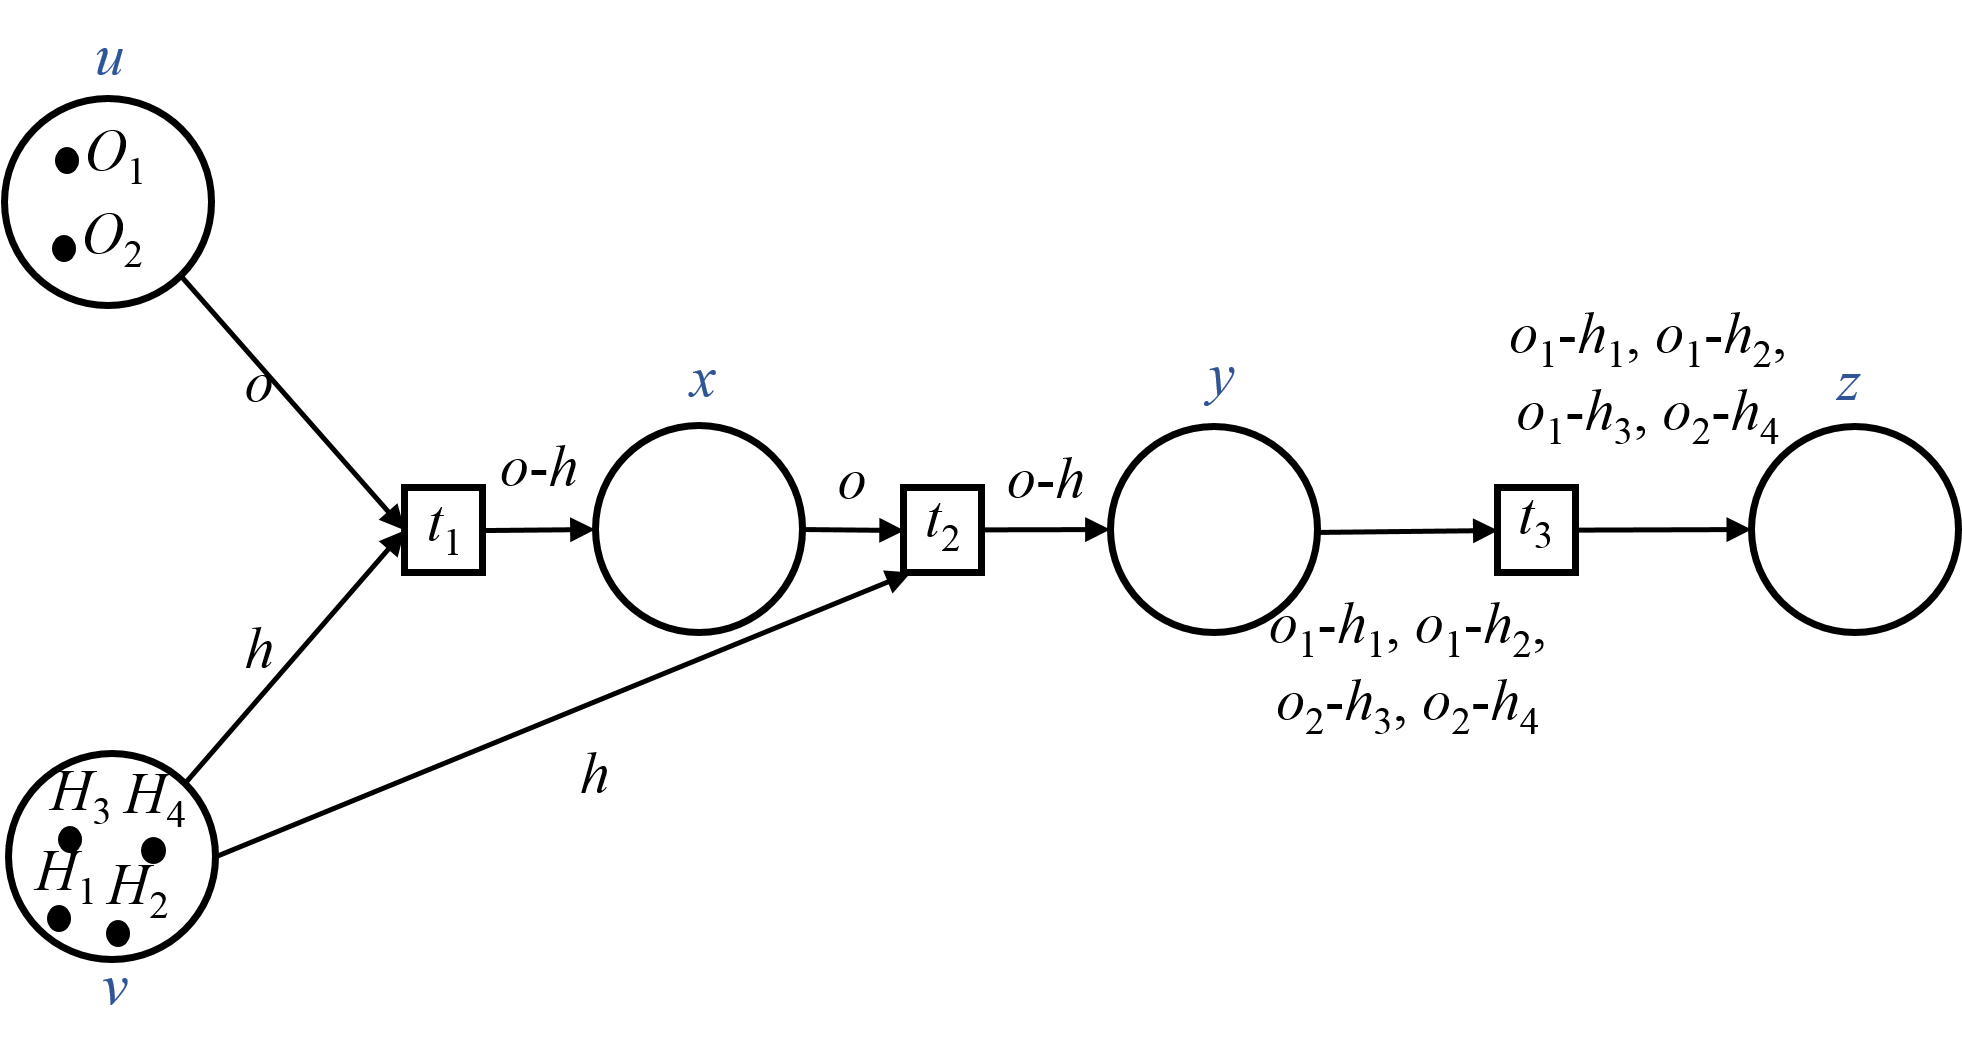
\includegraphics[width=8cm]{model.png}
	\caption{RPN model of the autoprotolysis of water}
	\label{RPNmodel}
\end{figure}

Fig.~\ref{RPNmodel} depicts the graphical representation of the RPN model for the autoprotolysis of water.
In this model, we assume two token types, $H$ for hydrogen
and $O$ for oxygen. They are instantiated via four token instances of $H$ ($H_1$, $H_2$, $H_3$, and $H_4$) and two token instances of
$O$, ($O_1$ and $O_2$). The net consists of five places and three transitions and the edges between
them are associated with token variables and bonds, where we assume that $\type(o)=\type(o_1)=\type(o_2) = O$
and $\type(h)=\type(h_1)=\type(h_2)=\type(h_3)=\type(h_4)=H$. 
Looking at the transitions, transition $t_1$ models the formation of a bond between a hydrogen
token and an oxygen token. Precisely, the transition stipulates a selection of two such
molecules with the use
of variables $o$ and $h$ on the incoming arcs of the transition which are bonded
together, as described in the outgoing arc of the transition.
Subsequently, transition $t_2$ completes
the formation of a water molecule by selecting an oxygen token from place $x$ and
a hydrogen token from place $v$ and forming a bond between them, placing the resulting component at place $y$. Note that the selected oxygen instance in this transition will be connected to a hydrogen token via a bond 
created by transition $t_1$; this bond is preserved and the component resulting from the creation of
the new $o-h$ bond will be transferred to place $y$. (Details about execution of the model will follow the
description of RPN semantics.)
Finally, transition $t_3$ models the autoprotolysis reaction: assuming the existence of two distinct oxygen
instances, as required by the variables $o_1$ and $o_2$ on the incoming arc of the transition, connected
with hydrogen instances as specified in $F(y,t_3)$, the transition breaks the bond $o_2-h_3$ and forms the
bond  $o_1-h_3$.  As such, assuming the existence of two water molecules at place $y$, the transition
will form  a hydronium  (H$_3^+$O) and a hydroxin (OH$^-$) molecule in place $z$ of the net.
The reversibility semantics of RPNs ensures that  reversing the transition $t_3$ will result in the re-creation
of  two water molecules placed at $y$, while the use of variables allows the formation of water molecules consisting
of different bonds between the hydrogen and oxygen instances, as will be explained in the sequel.


In order to introduce the semantics of RPNs we need to introduce some notations. Note that in 
the sequel we omit the discussion of negative tokens and negative bonds as they are not relevant to our
case study. We also restrict  our attention to causal reversibility which allows some simplifications
of the exposition and, in particular, of the history function defined below.
We write 
$\circ t =   \{x\in P\mid  F(x,t)\neq \emptyset\}$ and  
$ t\circ = \{x\in P\mid F(t,x)\neq \emptyset\}$
for the incoming and outgoing places of transition
$t$, respectively. Furthermore, we write
$\guard{t}  =   \bigcup_{x\in P} F(x,t)$ 
for the union of all labels on the
incoming arcs of  transition $t$, 
and $\effects{t}  =   \bigcup_{x\in P} F(t,x)$
for the union of all labels on the 
outgoing arcs of transition $t$. 
\begin{definition}\label{well-formed}{\rm 
		A \PN is \emph{well-formed}, if for all $t\in T$:
		\begin{enumerate}
			\item $A_V\cap \guard{t} = A_V\cap \effects{t}$,
			\item $ F(t,x)\cap F(t,y)\cap A_V=\emptyset$ for all $x,y\in P$, $x\neq y $. 
		\end{enumerate}
}\end{definition}
Thus, a \PN is well-formed if (1) whenever a variable exists in
the incoming arcs of a transition then it also exists on the outgoing arcs, which implies that transitions do not
erase tokens, and  (2) 
tokens/bonds cannot be cloned into more than one outgoing places.

As with standard Petri nets the association of token/bond instances to places is called a \emph{marking}  such that 
$M: P\rightarrow 2^{A_I\cup B_I}$, where we assume that if $(u,v)\in M(x)$ then $u, v\in M(x)$. 
In addition, we employ the notion of a \emph{history}, which assigns a memory to each
transition $H : T\rightarrow \mathbb{N}$. 
Intuitively, a history of $H(t) = 0$ for some $t \in T$ captures that the transition has not taken place, or 
every execution of it has been reversed, and a history
of $ H(t)=k, k>0$, captures that the transition was executed  $k$ times that have not been  reversed.
Note that $H(t)>1$ may
arise due to the consecutive execution of the transition with different token
instances. A pair of a marking and a history, $\state{M}{H}$, describes a \emph{state} of a RPN 
with $\state{M_0}{H_0}$ the initial state, where $H_0(t) = 0$ for all $t\in T$. 

Finally, we define $\connected(a_i,C)$, where $a_i\in A_I$ and $C\subseteq 2^{A_I\cup B_I}$,
to be the tokens connected
to $a_i$  as well as the bonds creating these connections according to 
set $C$. 

\paragraph{Forward Execution.}
During the forward execution of a transition in a RPN, 
a set of tokens and bonds, as specified by the incoming arcs of the transition, are selected and
moved to the outgoing places of the transition, as specified by the transition's outgoing arcs, possibly
forming or destructing bonds, as necessary. Given, however, the presence of multiple instances of the same token
type, it is possible that different token instances are selected during the transition's execution.  


A transition is forward-enabled in a state $\state{M}{H}$ of a \PN if there exists a selection of token instances 
available at the incoming places of the transition that 
match the requirements  on the transitions incoming arcs. Formally:

\begin{definition}\label{fenabled}{\rm
		Given a \RPN $(P,T, A, A_V, B, F)$, a state $\state{M}{H}$, and a transition $t$, we say that $t$ is 
		\emph{forward-enabled} in $\state{M}{H}$  if there exists a surjective function 
		$U:\guard{t}\cap A_V\rightarrow A_I$ such that:
		
		\begin{enumerate}
			\item  for all $v\in\guard{t}$, if $\type(v) = a$	then $\type(U(v))=a$
			\item for all $a\in F(x,t)$, then $U(a)\in M(x)$ and for all $(a,b)\in F(x,t)$, then $(U(a),U(b))\in M(x)$, 
			\item for all
			$(a,b)\in \effects{t}-\guard{t}$ then $(U(a),U(b))\not\in M(x)$ for all $x\in\circ t$.
		\end{enumerate}
}\end{definition}

Thus, $t$ is enabled in state $\state{M}{H}$ if  (1) there is a type-respecting assignment of token instances
to the variables on the incoming edges, with (2) the token instances originating from the appropriate
input places of the transition and  connected with
bonds as required by the variable bonds occurring on the incoming edges, and (3) if a bond
occurs in the outgoing edges of the transition but not the incoming ones, then the selected instances
associated with the bond's variables should not be bonded together in the incoming places
of the transition (thus transitions do not recreate bonds). We refer to $U$ as a forward enabling 
assignment.

To execute a transition $t$ according to an enabling assignment $U$, 
the selected token instances, along with their connected components,
are relocated to the outgoing places of the transition as specified
by the outgoing arcs, with bonds created and destructed accordingly. 
Furthermore,
the history of the executed transition is increased by one. Specifically,
we define:
\begin{definition}{\rm \label{forward}
		Given a \RPN $(P,T,  A, A_V, B, F)$, a state $\langle M, H\rangle$, and an
		enabling assignment $U$, we write $\state{M}{H}
		\trans{t} \state{M'}{H'}$
		where for all $x\in P$:
		\[
		M'(x) =   M(x)- \bigcup_{a\in f(x,t)} \connected(U(a), M(x)) 
		\cup  \bigcup_{a\in f(t,x),U(a)\in M(y)} \connected(U(a),S)\]
		where $S= (M(y)
		-\{(U(a),U(b))\mid (a,b)\in F(y,t)\})\cup \{ (U(a),U(b))\mid (a,b)\in F(t,x) \}$
		\[
		\hspace{0.2in}\mbox{and}\hspace{0.2in}
		H'(t') = \left\{
		\begin{array}{ll}
		H(t')+1, \hspace{1cm} \textrm{ if } t' = t  \; \\
		H(t'), \hspace{1.5cm}  \;\textrm{ otherwise }
		\end{array}
		\right.			\]	
}\end{definition} 


\paragraph{Reversing Execution.}
We now move on to  reversing transitions. 
A transition can be reversed in a certain state if it has been previously executed and there exist token instances in its output places 
that match the requirements on its outgoing arcs. Specifically, we define the notion of reverse enabledness
as follows.
\begin{definition}\label{renabled}{\rm
		Consider a \RPN $(P,T, A, A_V, B, F)$, a state $\state{M}{H}$, and a transition $t$.
		We say that $t$ is \emph{reverse-enabled} in $\state{M}{H}$ if (1)  $H(t)\neq 0$, and (2)
		there exists a surjective function 
		$W:\effects{t}\cap A_V\rightarrow  A_I$ such that:
		\begin{enumerate}
			\item  for all
			$v\in\effects{t}$, if $\type(v) = a$
			then $\type(W(v))=a$, 
			\item for all $a\in F(t,x)$, then $W(a)\in M(x)$ and for all $(a,b)\in F(t,x)$, then $(W(a),W(b))\in M(x)$, 
			\item  for all $(a,b)\in \guard{t} - \effects{t}$ then $(W(a),W(b))\not\in M(x)$ for all $x\in\circ t$.
		\end{enumerate}
}\end{definition}

Thus, a transition $t$ is reverse-enabled in $\state{M}{H}$ if  
(1) the transition has been executed and (2) there exists a type-respecting assignment of token instances,
from the instances in the out-places of the transition, to the variables on the outgoing
edges of the transition, and where the instances are connected with bonds as required by
the transition's outgoing edges.  Also we do not recreate bonds when going backwards. 
We refer to $W$ as a reversal enabling assignment.
To implement the reversal of a transition $t$ according to a reversal enabling assignment $W$, 
the selected instances are relocated from  the outgoing places of the transition to the incoming places,
as specified
by the incoming arcs of the transition, with bonds created and destructed accordingly:

\begin{definition}\label{causal}{\rm
		Given a \RPN $(P,T, A, A_V, B, F)$, 
		a state $\langle M, H\rangle$, and a transition $t$ reverse-enabled in $\state{M}{H}$  with 
		$W$ a reversal enabling assignment, we write $ \state{M}{H}
		\rtrans{t} \state{M'}{H'}$   where for all $x$:
		\[
		M'(x) =   M(x)- \bigcup_{a\in f(t,x)} \connected(W(a), M(x)) 
		\cup  \bigcup_{a\in f(x,t),W(a)\in M(y)} \connected(W(a),S)\]
		where $S= (M(y)
		-\{(W(a),W(b))\mid (a,b)\in F(t,y)\})\cup \{ (W(a),W(b))\mid (a,b)\in F(x,t) \}$
		\[
		\hspace{0.3in}\mbox{and}\hspace{0.3in}
		H'(t') = \left\{
		\begin{array}{ll}
		H(t') - 1, \hspace{0.3cm} \;\;\textrm{ if } t' = t  \; \\
		H(t'),\hspace{1cm}  \;\textrm{ otherwise }
		\end{array}
		\right.
		\]
}\end{definition}	
\begin{figure}
	\centering
	%\subfigure{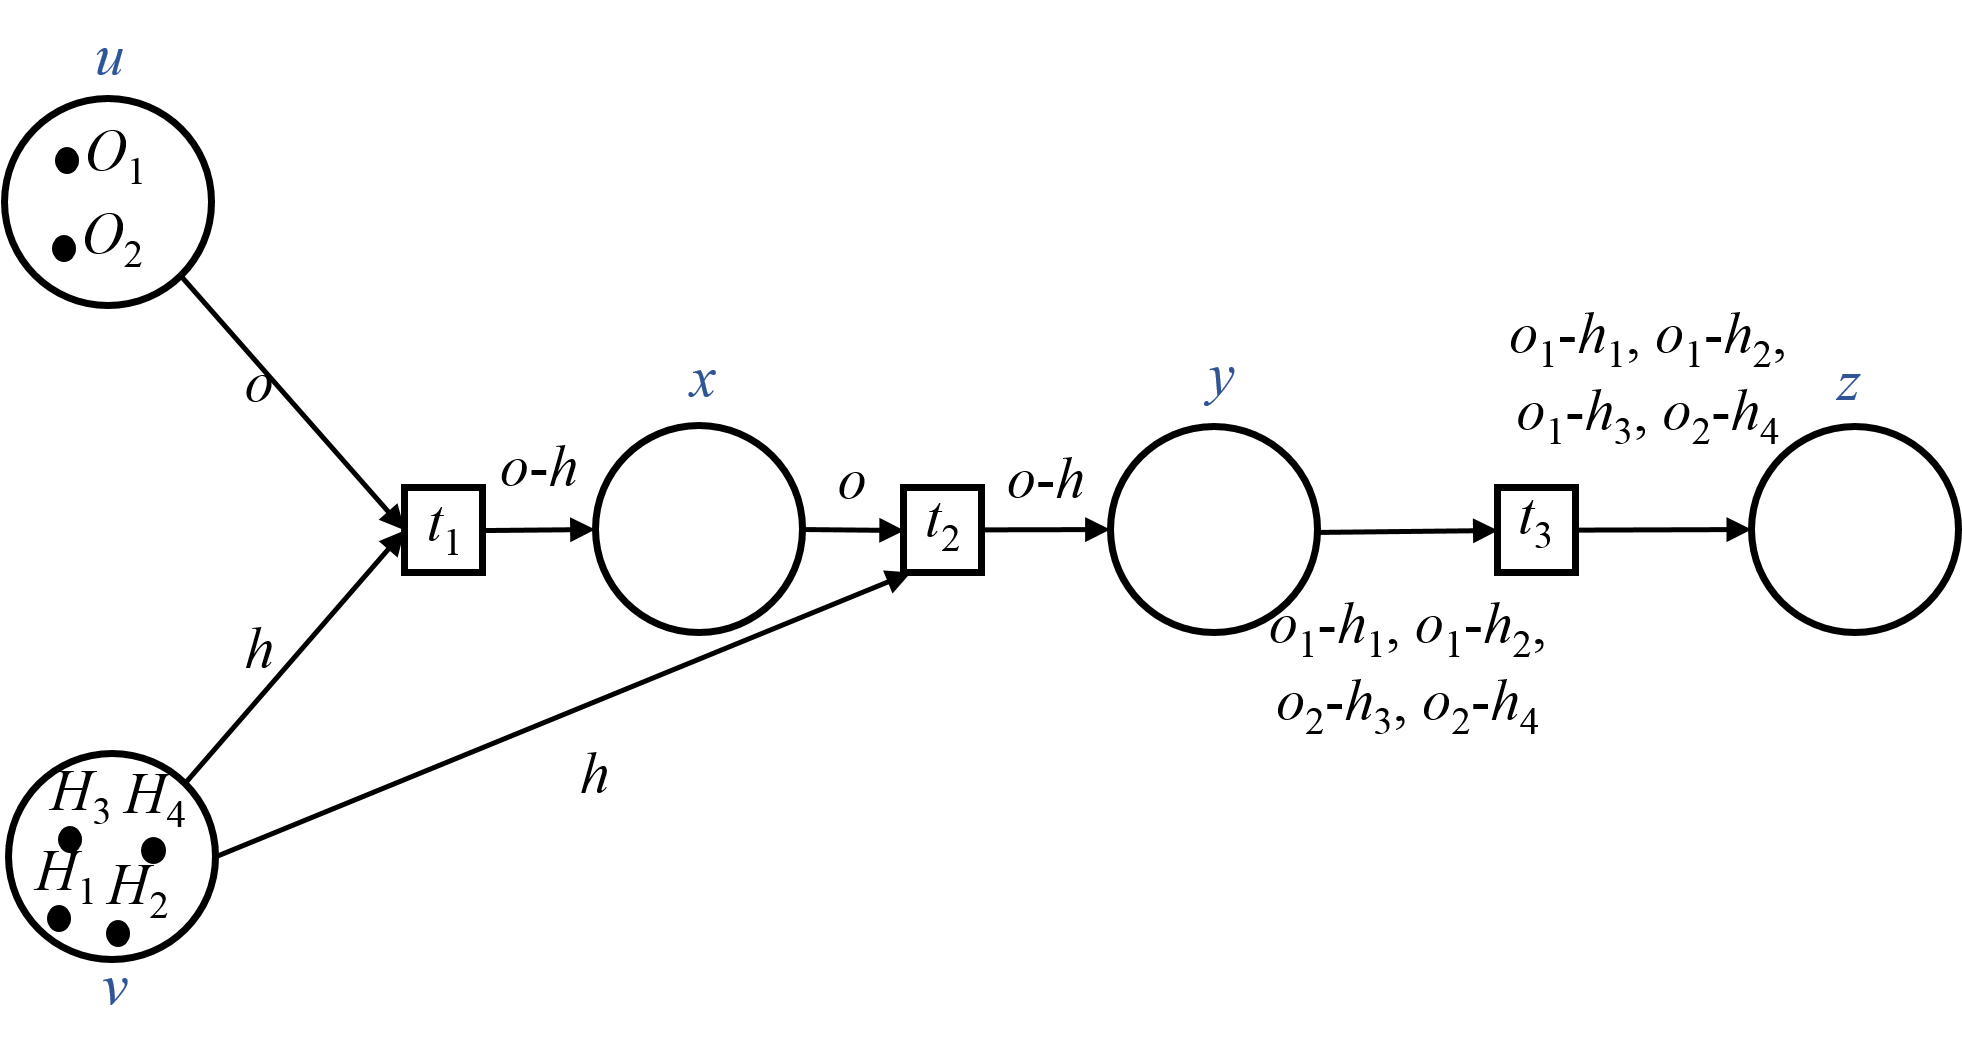
\includegraphics[width=6.3cm]{model.png}}
	\subfigure{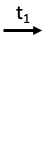
\includegraphics[width=.5cm]{arrowt1.png}}
	\subfigure{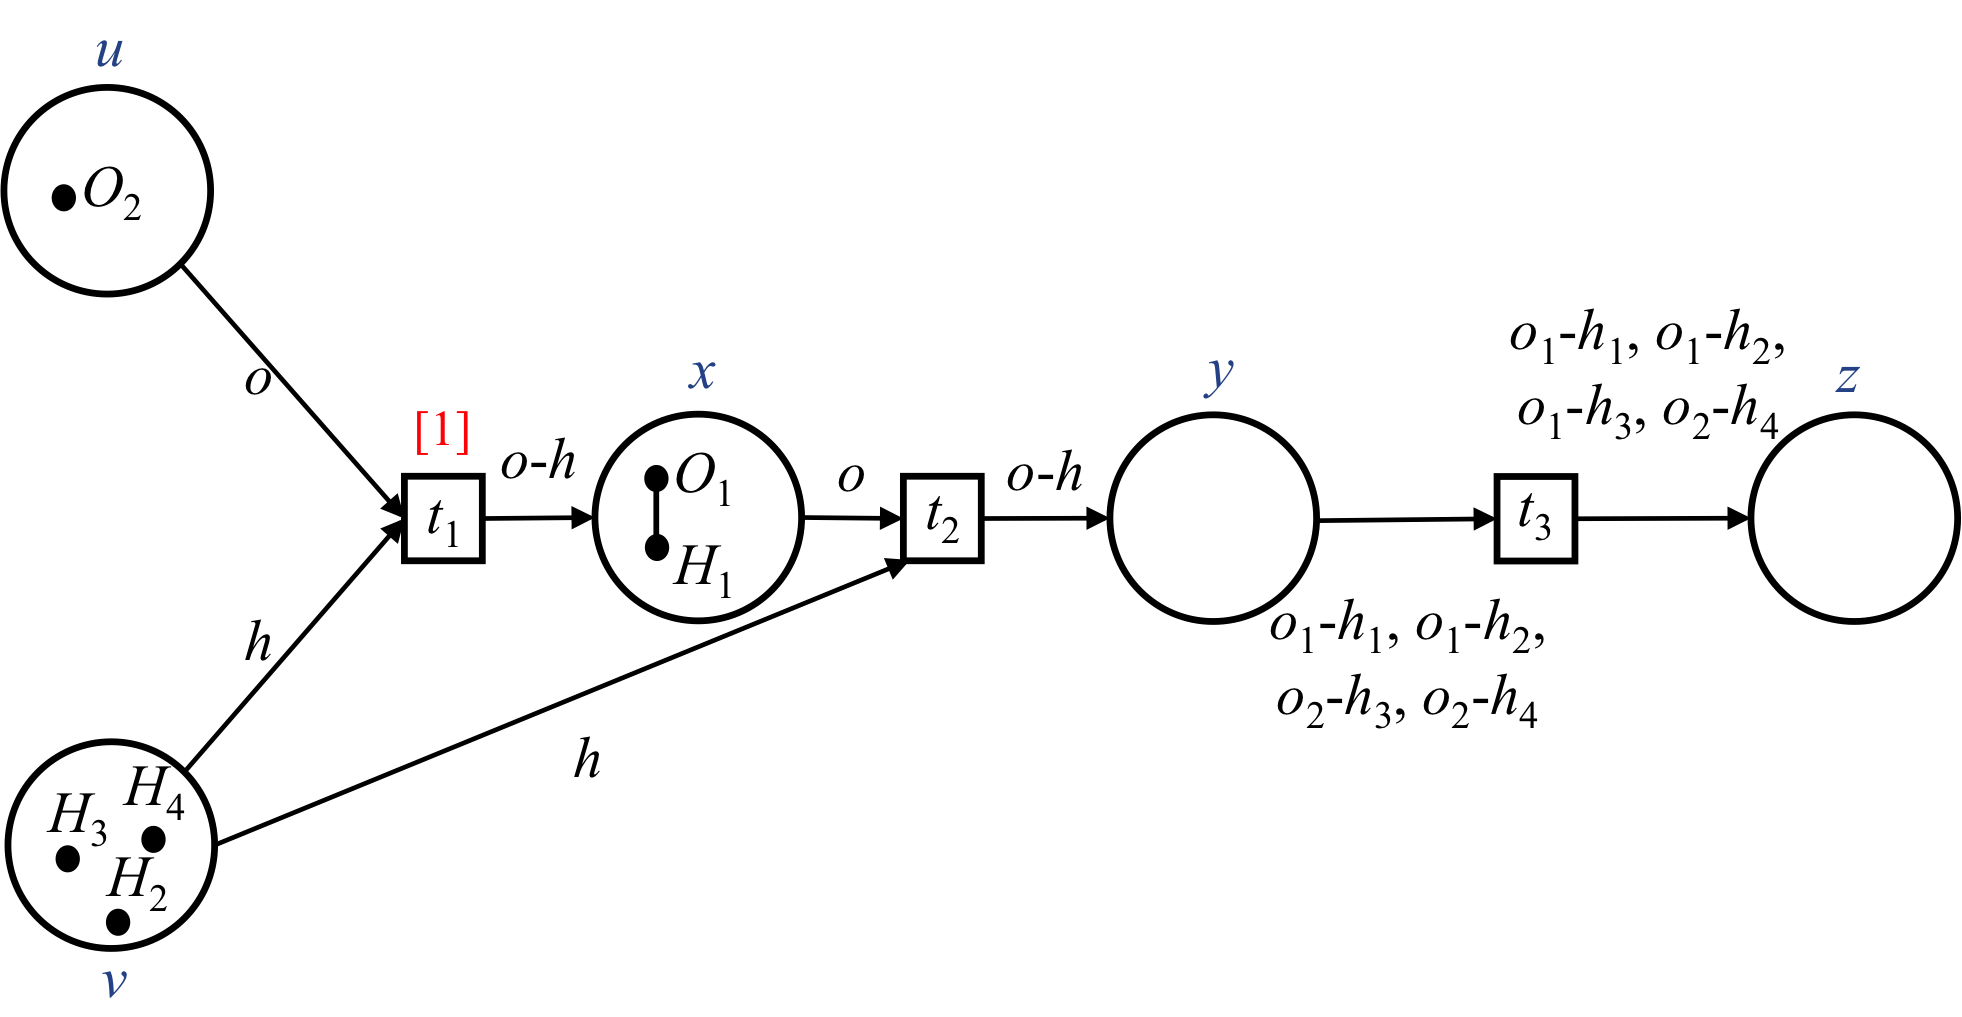
\includegraphics[width=7.2cm]{aftert1.png}}\\\vspace{-0.25cm}
	\subfigure{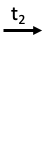
\includegraphics[width=.5cm]{arrowt2.png}}
	\subfigure{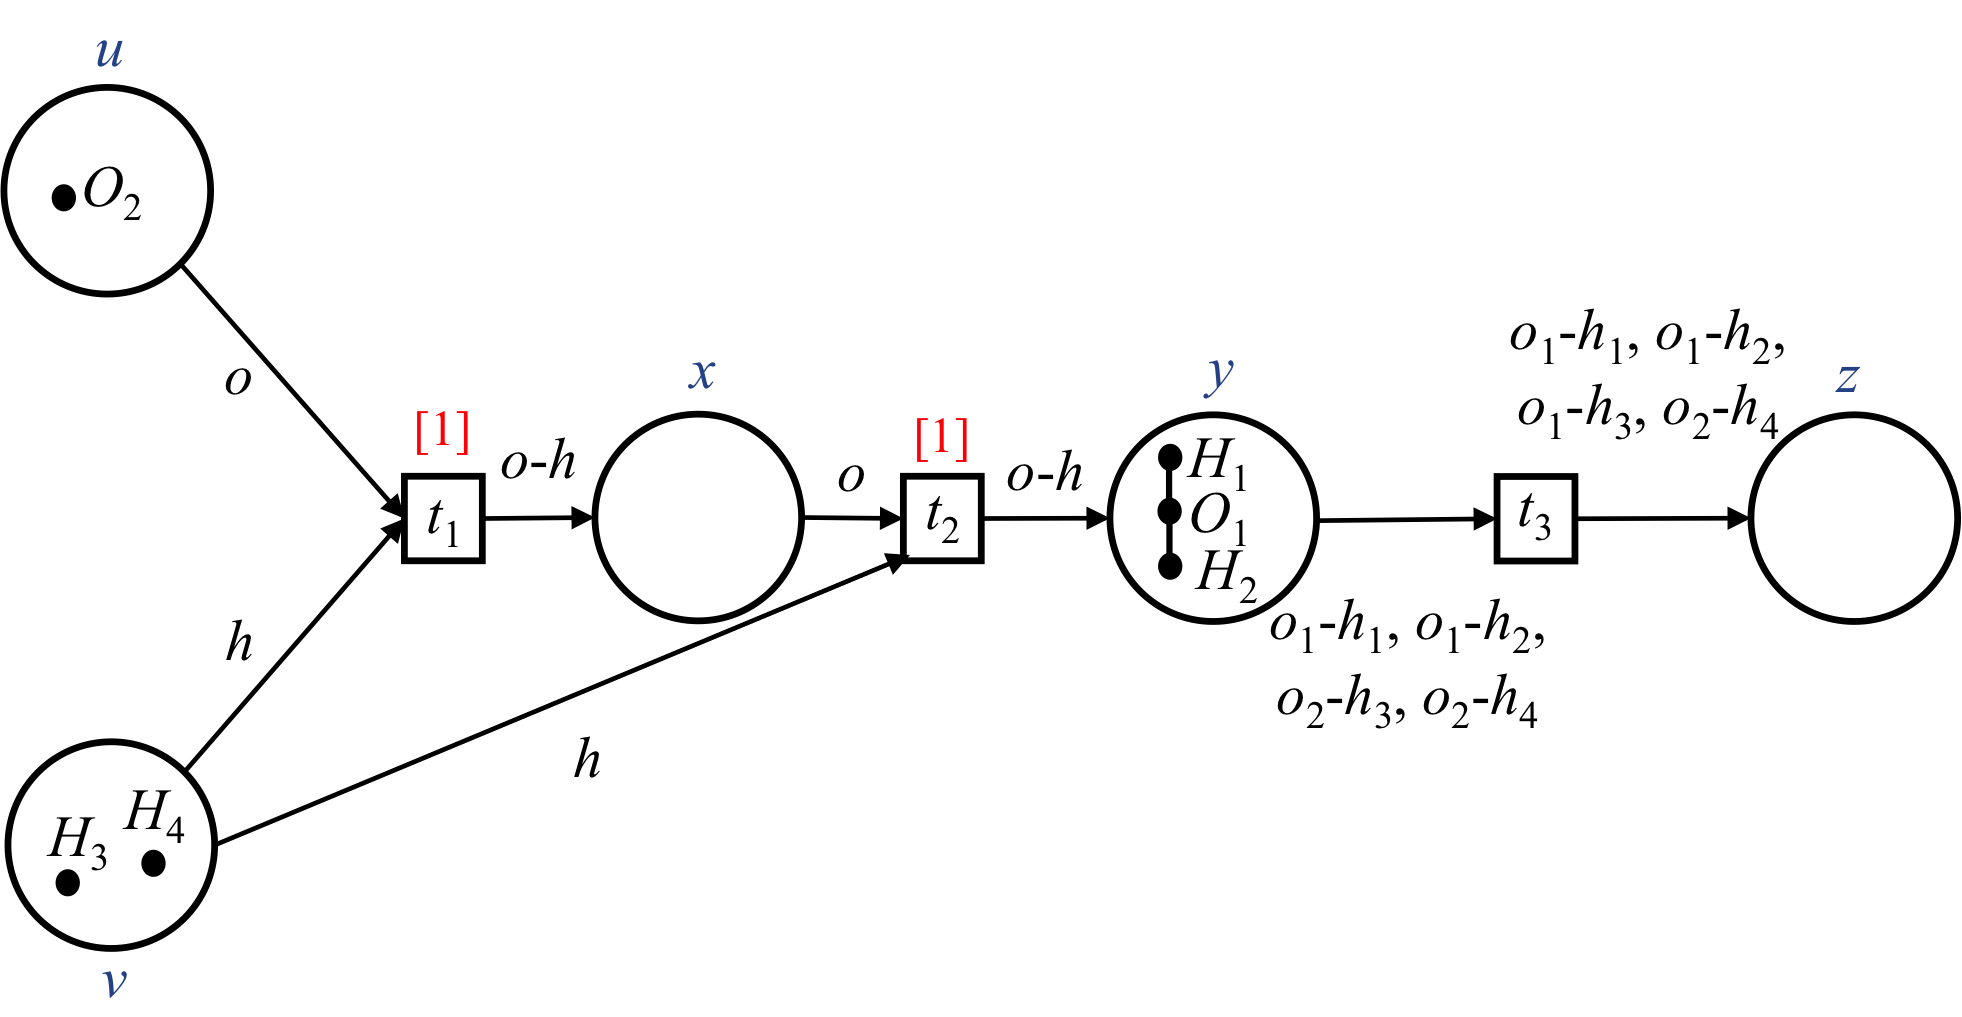
\includegraphics[width=7.2cm]{aftert2.png}}\\\vspace{-0.25cm}
	\subfigure{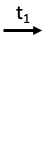
\includegraphics[width=.5cm]{arrowt1.png}}
	%\subfigure{\includegraphics[width=6.6cm]{aftert12.png}}
	\subfigure{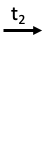
\includegraphics[width=.5cm]{arrowt2.png}}
	\subfigure{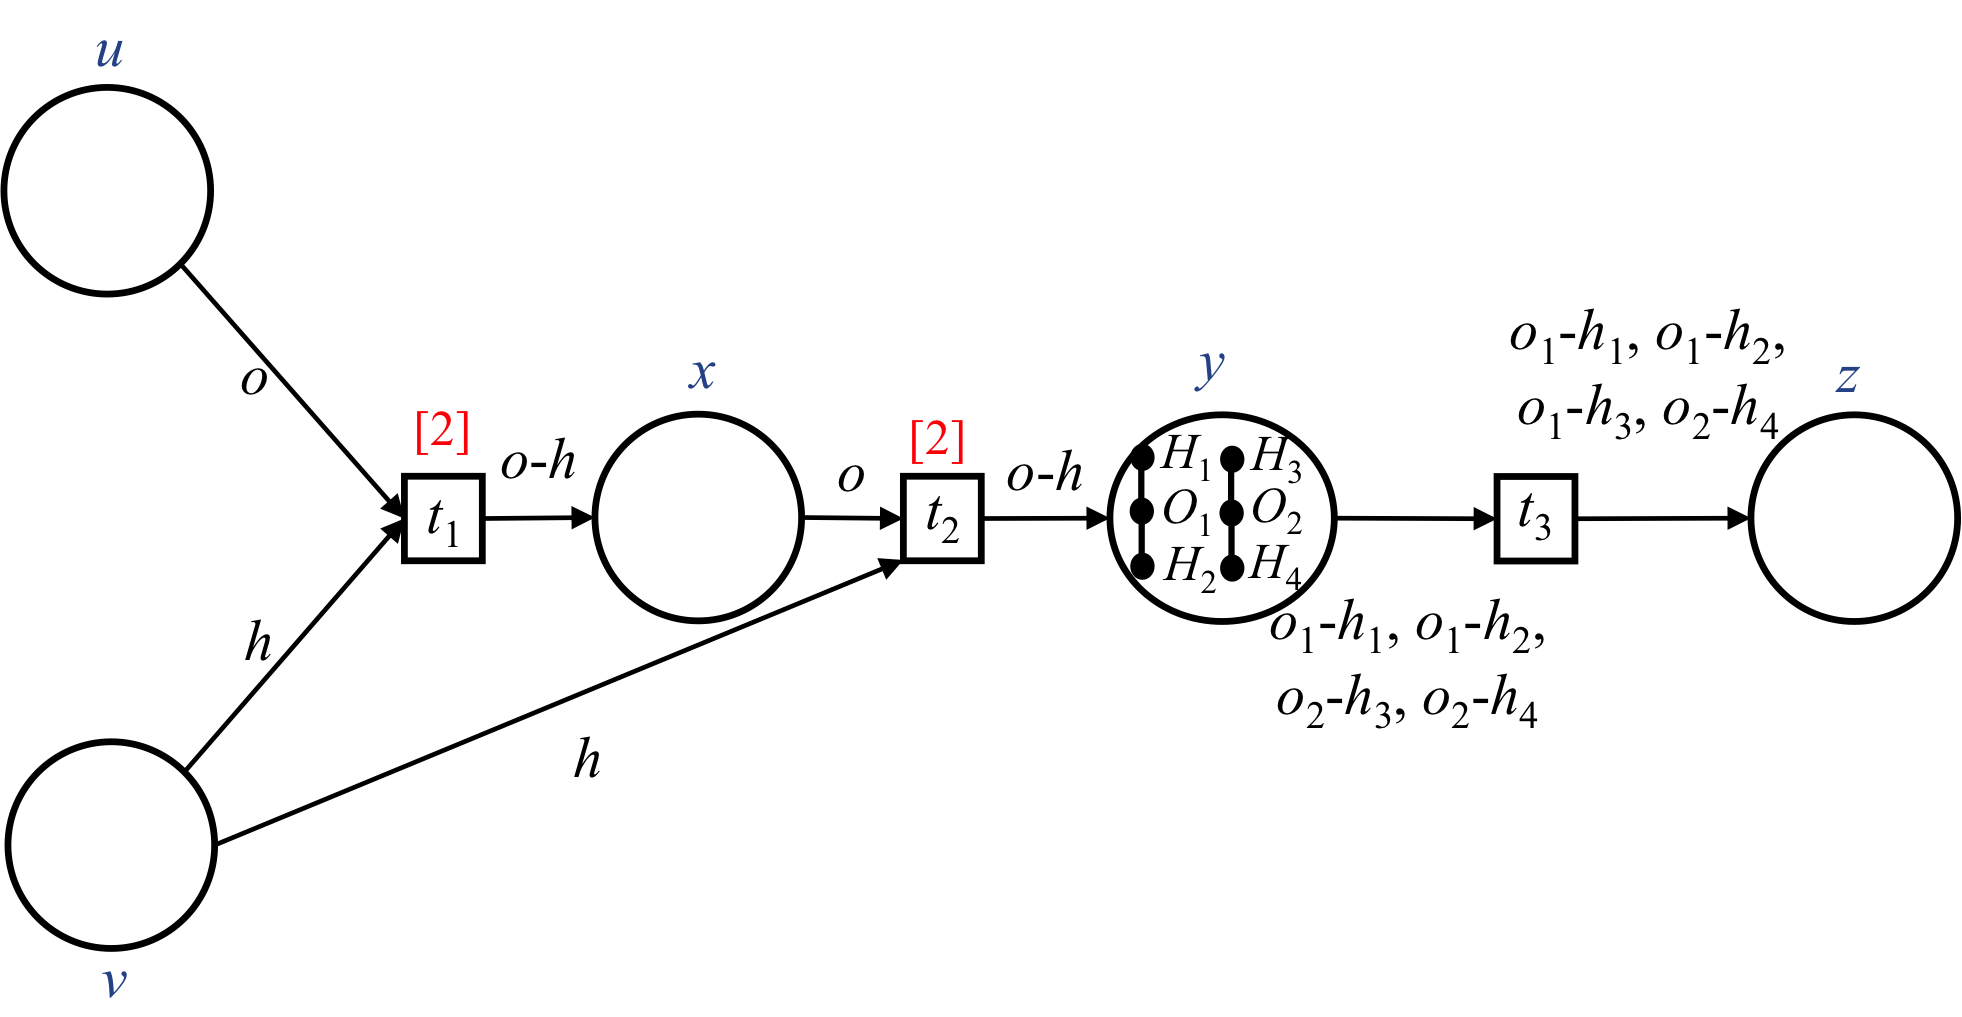
\includegraphics[width=7.2cm]{aftert22.png}}\\\vspace{-0.25cm}
	\subfigure{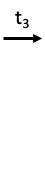
\includegraphics[width=.5cm]{arrowt3.png}}
	\subfigure{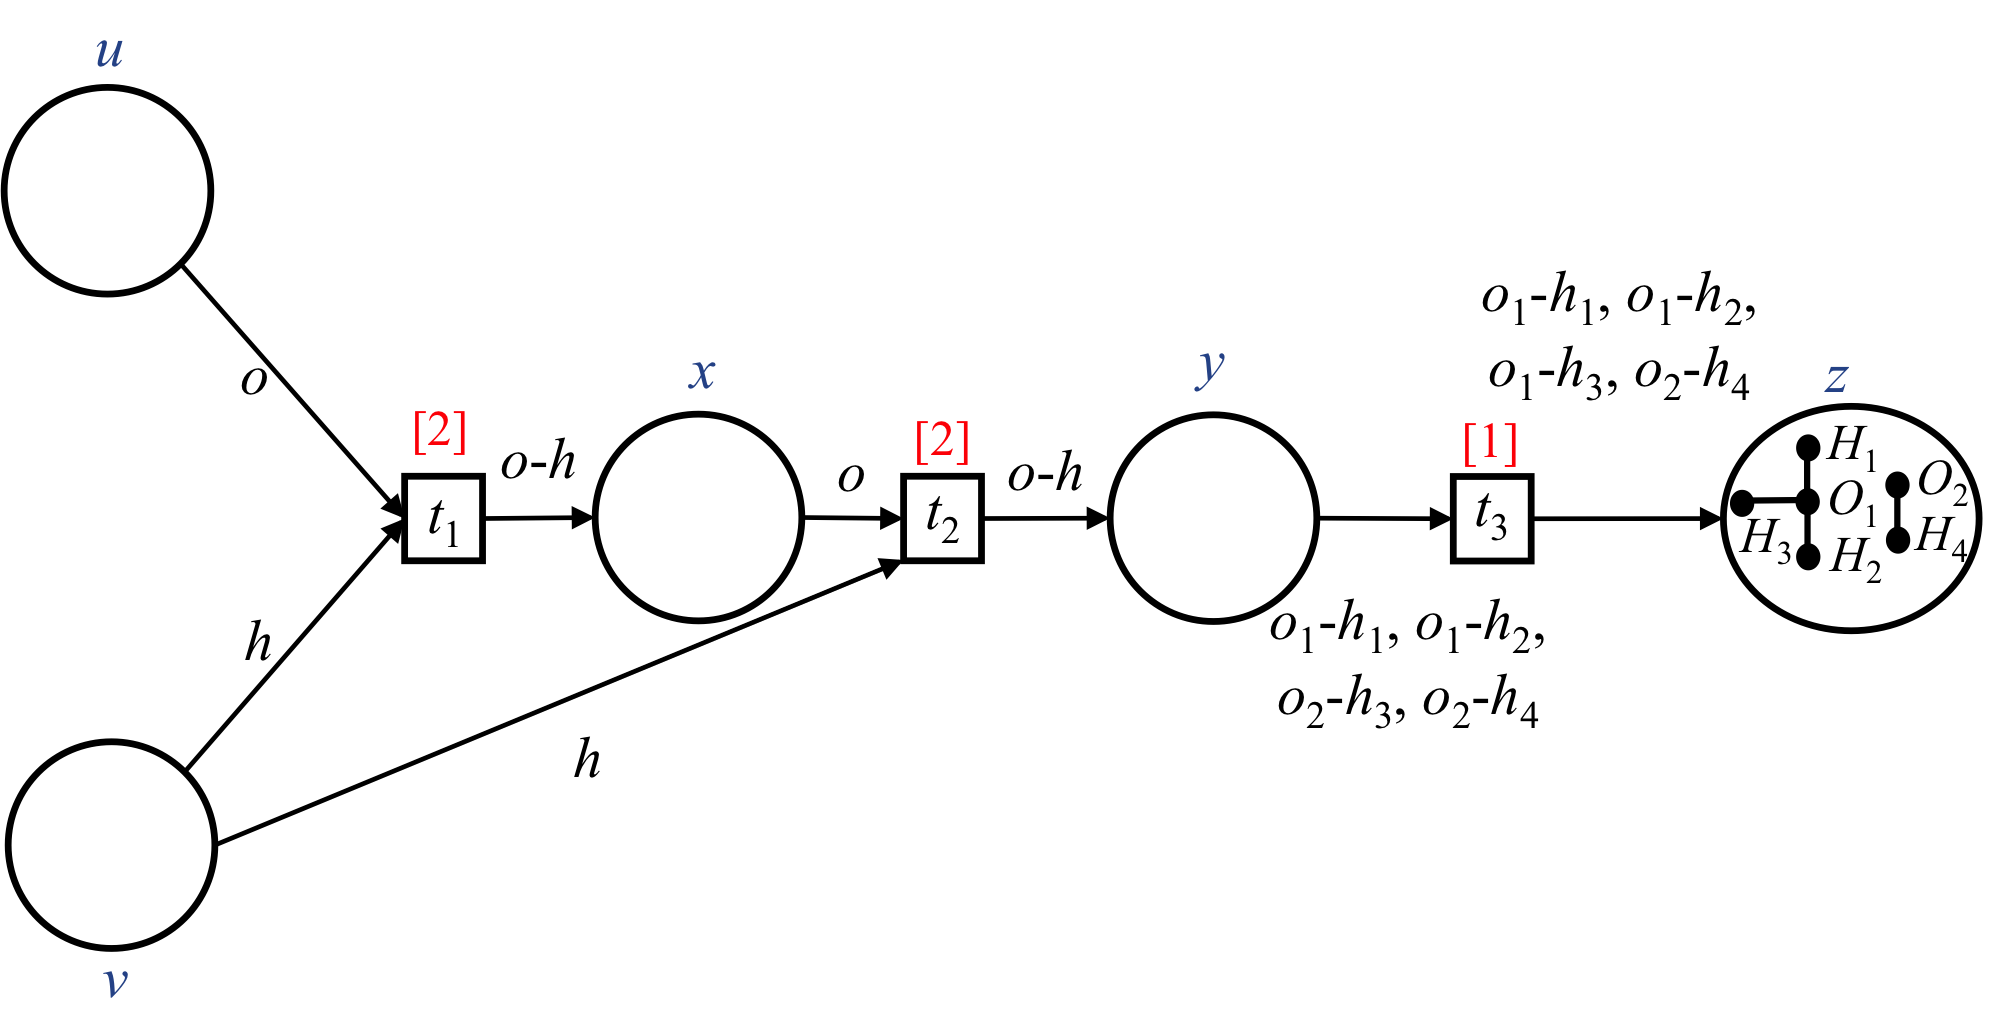
\includegraphics[width=7.2cm]{aftert3.png}}\\\vspace{-0.25cm}
	\subfigure{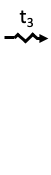
\includegraphics[width=.5cm]{arrowt3r.png}}
	\subfigure{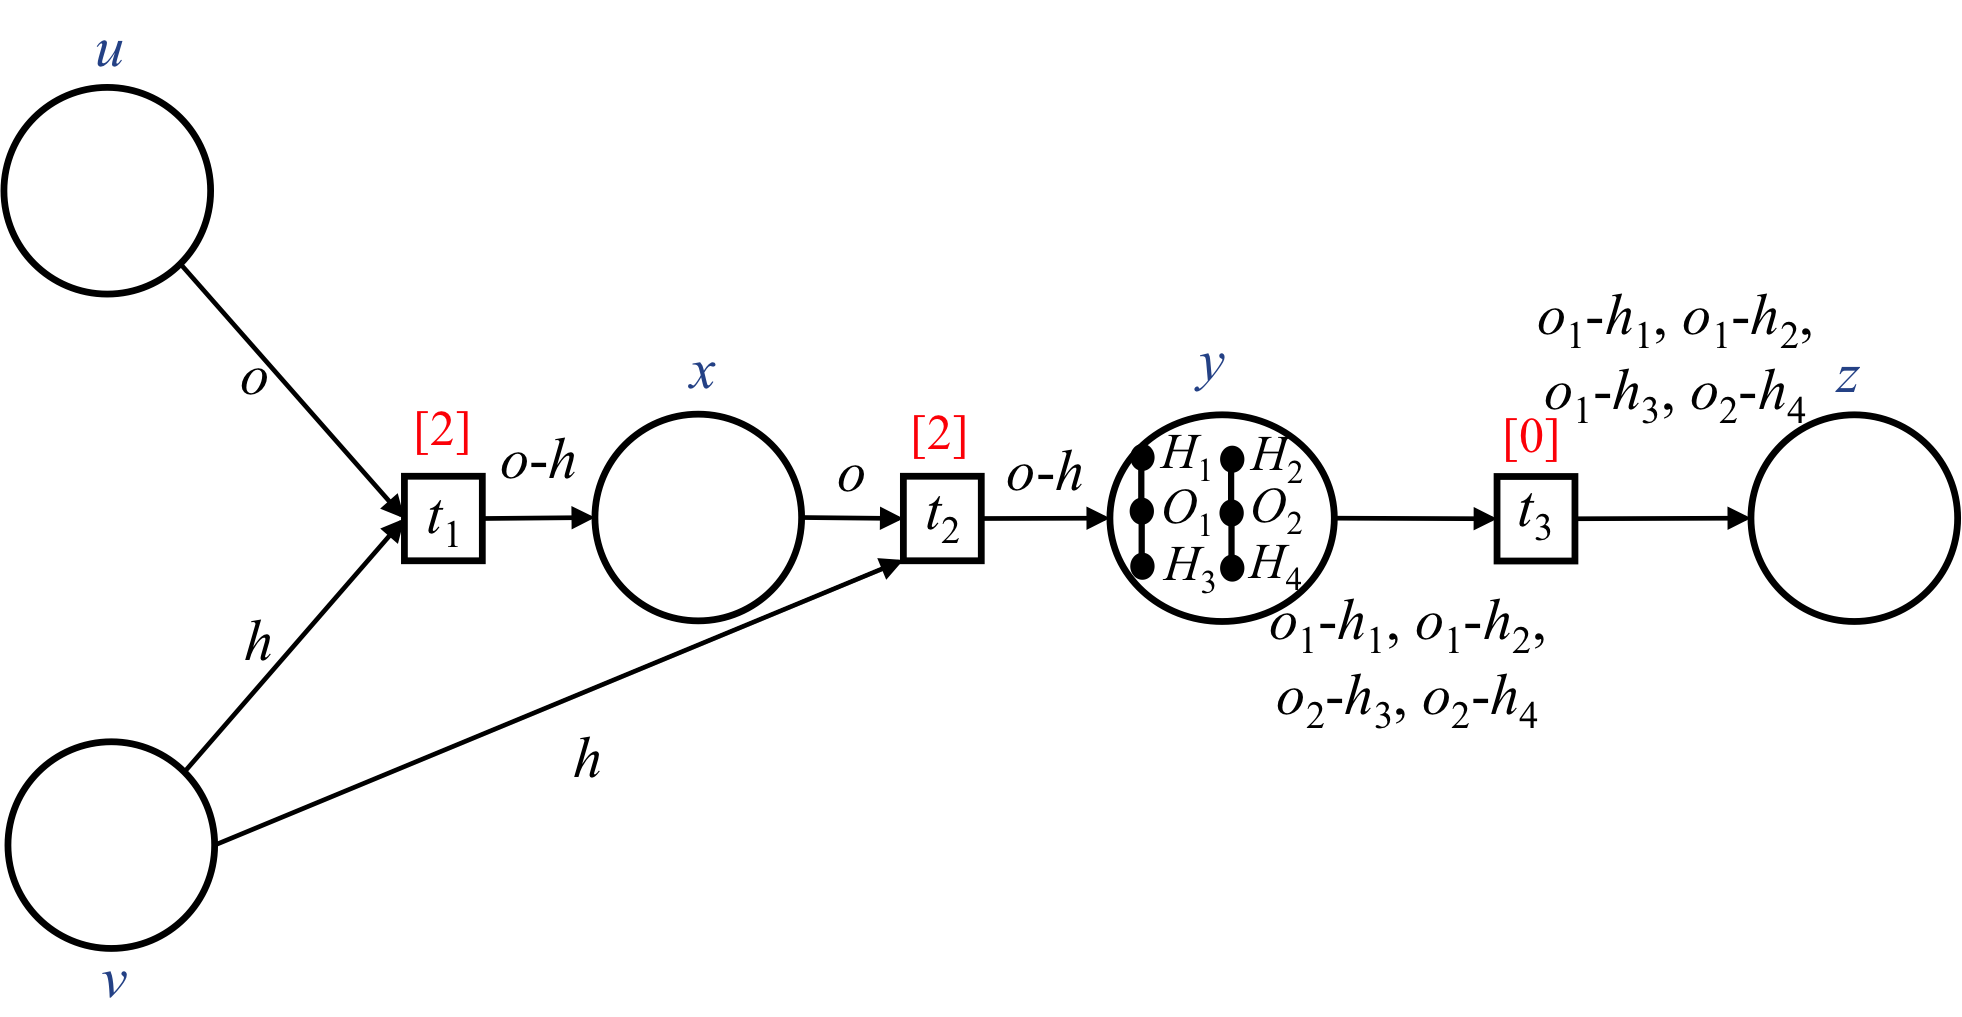
\includegraphics[width=7.2cm]{aftert3r.png}}
	\caption{Execution of the RPN autoprotolysis of water model.}
	\label{execution}
\end{figure}

We now return to the RPN autoprotolysis model and in Fig.~\ref{execution} we present
a possible execution of the model. The first net in this sequence shows the system after 
the execution of transition $t_1$ with enabling assignment $U(h)=H_1, U(o)=O_1$. Note
that the term $[1]$ written over transition $t_1$ captures that at this point $H(t_1)=1$ 
since the transition has been executed once.
This notation is generally used for histories in the graphical representation with occasional
missing histories corresponding to histories equal to $0$.
Subsequently,
we have the model after execution of transition $t_2$ with enabling assignment $U(h)=H_2,
U(o)=O_1$, creating the bond $O_1-H_2$, thus forming the first water molecule. A second
execution of transitions $t_1$ and $t_2$ results in the second molecule of water in the system,
placed again at place $y$, as shown in the third net in the figure. At this state, transition
$t_3$ is forward-enabled and,  with enabling assignment $U(o_1)=O_1, U(o_2)=O_2, U(h_1)=H_1, 
U(h_2)=H_2,U(h_3)=H_3,U(h_4)=H_4$, we have the creation of the hydronium and hydroxide
depicted at place $z$ in the fourth net of the figure. At this stage  transition $t_3$ is
now reverse-enabled and the last net in the figure illustrates the state resulting after
reversing $t_3$ with reversal enabling assignment $W(o_1)=O_1, W(o_2)=O_2, W(h_1)=H_1, 
W(h_2)=H_3,W(h_3)=H_2,W(h_4)=H_4$.


\section{Conclusion}

We have presented three formalisms to model chemical reactions. In CCB, we can model a simple covalent chemical reaction. In particular, when modelling the autoprotolysis of water, we can include the concerted reaction and we can model that the reverse reaction can work on any of the hydrogens, not just the one transferred in the forward step. The same modelling of hydrogens and oxygens can be used to model a more complex reaction, involving carbon atoms as well \cite{KUHN201818}. This shows that the modelling implements general concepts and not only this particular situation. CCB can also be used to model situations beyond simple chemical reactions  \cite{merevcomp2018}. As mentioned, the reverse reaction can work by transferring any of the hydrogens of the hydronium. In our calculi, we can actually distinguish the hydrogens due to the subscripts used. When reversing the reaction in CCB, instead of the transition in Section~\ref{sec:ccb}, we could also have done this (writing the transition and the rewrite together):
%
\begin{flalign*}
&(( (h_1[1];p).H'_1 \paral (h_2[2];p).H'_2 \paral (o_1[1],o_2[2],n[5]).O'_1) \paral (h_3[5];p).H'_3) &&\\
&\paral (h_4[4];p).H'_4  \paral (o_3,o_4[4],n).O'_2&&\\
&\xrightarrow{\{ np[3], \underline{nh_{1}}[1]\}} \Rightarrow &&\\
&(( (\boldsymbol{h_1[3]};p).H'_1 \paral (h_2[2];p).H'_2 \paral (\boldsymbol{o_1[5]},o_2[2],\boldsymbol{n}).O'_1) \paral (h_3[5];p).H'_3) &&\\
&\paral (h_4[4];p).H'_4  \paral (\boldsymbol{o_3[3]},o_4[4],\boldsymbol{n}).O'_2
\end{flalign*}
%
The result is different from that in Section~\ref{sec:ccb}, but identical from a chemical point of view, since the hydrogens are all identical. On the other hand a technique called isotopic labelling can be used to trace atoms by using different isotopes of, in this case hydrogen, confirming that the different options happen in reality. 

The bonding calculus is a process calculus suitable for modelling in a natural way the dynamics of the interactions in biochemical systems. It is suitable for describing appropriate compositions between several molecules (e.g., hydrogen, oxygen and carbon). In bonding calculus each molecule has a unique name, while the bonds between molecules can be of the same type and have identical names. The bonding calculus is compositional, and so it can explicitly describe the activity of a complex system by composing the activities of its components. The direction of the evolution (forward and reverse) depends on the execution of either bond and unbond actions, and can be controlled only if the choice operator is not used. Simulations by using a software platform can be used to analyze the dynamics of the bonding systems, allowing to test the validity of some underlying assumptions. Moreover, we can verify various properties of the bonding compounds described by using the calculus.


Reversing Petri Nets are Petri net structures that assume tokens to be distinct and persistent where during the execution of transitions tokens can be bonded/unbonded with each other, and the creation of these bonds is considered to be the effect of a transition, whereas their destruction/creation is the effect of the transition’s reversal. Reversing Petri nets are a natural choice to model and analyse biochemical reaction systems, such as the autoprotolysis of water, which by nature
has multi-party interactions, is inherently concurrent, and features reversible behaviour. 
In particular, the feature of token multiplicity and
the use of variables allows to non-deterministically
select different combinations of atoms of a particular element when creating molecules. Also the possibility for
transitions to break bonds allows to model concerted actions where a transition simultaneously
destructs  a water molecule and creates a hydronium whose  reversal results in the opposite effect. Furthermore,
the collective token interpretation adopted in the framework, treating all tokens of the same type
as equivalent, allows the reaction to reverse into two different water molecules than the original ones,
i.e., using different instances of the atoms.
Note that the presented model abstracts away the positive/negative charge of the atoms and
captures the existence of electrons by the enablednes of transitions. A model at a lower
level of abstraction would be possible by introducing tokens to represent the electrons  bonded to the associated
atom tokens to illustrate the relevant charges. 

Reversing Petri nets are a general purpose model where their expressiveness offers the ability to model 
a variety of distributed systems other than biochemical reactions. In particular, they have been used successfully for
the modelling of a transaction-processing system~\cite{RPNs}, and a novel antenna selection  algorithm~\cite{RC19}. 
Their extension in~\cite{RC19} also introduces
a mechanism for controlling reversibility 
 that may capture environmental or other conditions that determine a transition's
reversal, e.g., changes in temperature. In future work, we plan to exploit recent work that establishes a translation of a subclass of RPNs to coloured Petri nets~\cite{RPNtoCPN} towards the development of a methodology for the analysis of reversing Petri nets exploiting available tools.

Considering the three formalisms mentioned, all can represent this reaction. CCB is quite close to the chemical concepts and can therefore model this reactions faithfully. In particular, it shows the linked forming and breaking of bonds. In the Bonding Calculus, this link is not expressed. All models avoid a $H_3O^+$ molecule forming directly. All models presented use subscripts and enable the tracking of atoms. We can see that the Bonding Calculus is restricted because the reverse reaction must transfer exactly the hydrogen used in the forward reaction. 

\addcontentsline{toc}{chapter}{Bibliography}

\bibliography{springer}{}
\bibliographystyle{splncs04}

\end{document}
